%\chapter{det-overview}

%%%%%%%%%%%%%%%%%%%%%%%%%%%%%%%%%%%%%%%%%%%%%%
\section{Detector Requirements}\label{sec:detector_requirements}

insert detector overview here \fixme{The whole chapter is `overview'; insert detector requirements here! Link added.}

%%%%%%%%%%%%%%%%%%%%%%%%%%%%%%%%%%%%%%%%%%%%%%
\section{Liquid argon detector properties}
- Electron drift + LAr purity etc.
- LAr scintillation light 

%%%%%%%%%%%%%%%%%%%%%%%%%%%%%%%%%%%%%%%%%%%%%%
\section{TPC Signal Formation}\label{sec:tpc_signal_formation}


The principle of a large single-phase LArTPC with wire readout is shown in 
Figure~\ref{fig:signal}. When charged particles traverse the LAr,
ionization electrons are generated. They %would 
travel at a constant speed 
($\sim$1.6 km/s at 500~V/cm electric field) along the electric field 
toward the anode plane assembly (APA) which consists of multiple anode wire planes. 
The first two wire planes encountered collect 
an induction signal as the drifting charges pass through.  The charge is collected 
on the wires of the third plane. The transparency of the induction planes is assured by 
applying appropriate bias voltages to all three wire planes. As charges drift pass the induction 
plane wires and are collected on the anode wires
a current is produced on the wires. Since the locations of all wires are 
accurately known, the position of the ionization charge in the direction 
transverse to the drift can be determined in three independent views. The time 
of the initial interaction can be determined by collecting scintillation light 
in a fast optical detector system. By measuring the time from the light signal 
to electrical signals on the wires, it is possible to determine the longitudinal position 
along the drift direction, leading to %. Therefore, one can achieve 
a 3D image of the trajectories 
of the charged particles in the LAr. The amount of ionization electrons depends on 
the energy and type of the initial particles, and can be used to deduce their properties.

\begin{cdrfigure}[The principles of LArTPC technology]{signal}{The principles of LArTPC technology are shown. (left) When energetic, charged particles 
traverse the LAr medium, ionization electrons are produced and move
along the external electric field towards the anode planes. (right) The ionization
electrons pass through the induction wire planes and are  collected by the 
final collection wire plane. 
During this process, signals are measured on the wires
in each plane which provides information about the 3D positions and
energies of initial particles.}
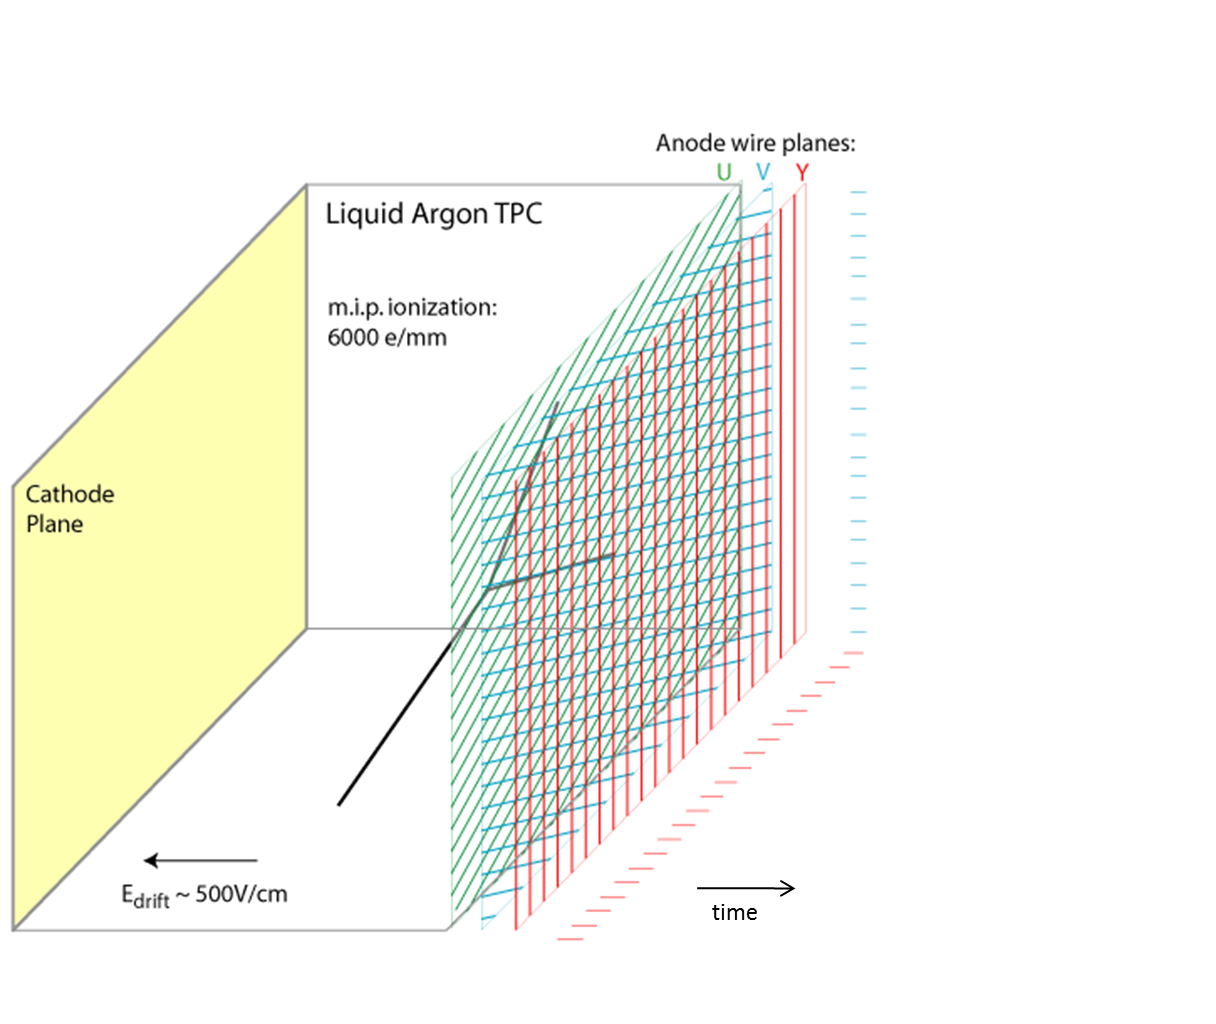
\includegraphics[width=0.48\textwidth]{TPC_1.png}
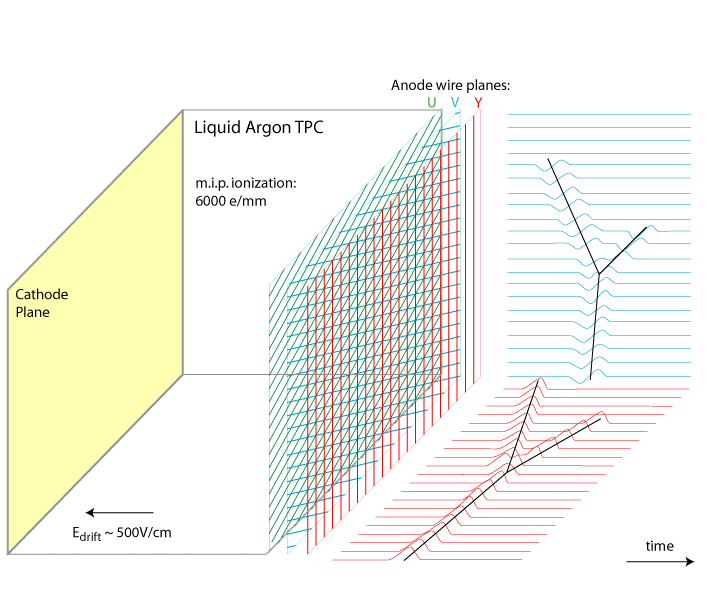
\includegraphics[width=0.48\textwidth]{TPC_2.png}
\end{cdrfigure}


Figure~\ref{fig:signal_formation} illustrates the major elements of the processes 
involved in forming the TPC signals. When the ionization electrons drift through the 
wire planes, current is induced on the nearby wires. This process is described by the 
field response functions. The physics of the current induction is described by the 
Shockley-Ramo theorem~\cite{Shockley,Ramo}.  For an element of ionization charge, 
the instantaneous, induced current $i$ is proportional to the amount of that
charge $q$: 
\begin{equation}
i = q \cdot \vec{E}_{w} \cdot \vec{v}_q.
\end{equation}
The proportionality factor is product of the weighting field vector $\vec{E}_{w}$ 
at the location of the charge and its drift velocity vector $\vec{v}_q$. 
The weighting field vector $\vec{E}_{w}$, which depends on the geometry of the electrodes, 
can be calculated by removing the charge,  placing the potential of the targeted 
electrode to the unity potential, and setting all other conductors to ground. 
Figure~\ref{fig:signal_formation} shows a calculated weighting potential 
\fixme{the `weighting potential' is E dot v? If so, please state that here}
for one 
induction plane wire using a 2D simulation based on Garfield~\cite{garfield}. 
In this calculation, the wire pitch is assumed to be 3~mm. There are three wire planes 
with the first two being induction and the last one being collection plane.  

The induced current on the wire is received, amplified, and shaped by
a pre-amplifier. This part is described by the electronics response
function (see Figure~\ref{fig:ele_res}).  
The resulting signal waveform is then digitally sampled at
regular intervals.  This data is referred to as the raw digits.  The
goal of the charge extraction process is to recover the number of
ionization electrons that must have arrived at each anode plane at a
given sample time in order to produce the measured raw digits.  The
information regarding the number, location (in the directions transverse
to and in the plane of the wires) and sample time of ionization
electrons are then used as input to the event reconstruction chain.

\begin{cdrfigure}[The process of TPC signal formation.]{signal_formation}{The process of TPC signal formation (left). The panel on the 
right shows a cross sectional view of the three wire planes (red dots) along with the electric field (orange lines) and the weighting potential 
(green lines) for a single induction wire of the first induction wire plane.}
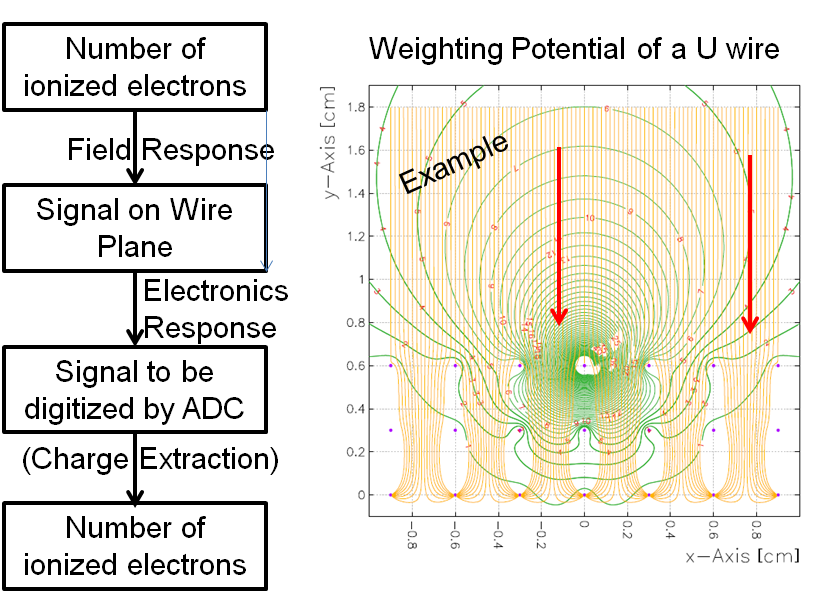
\includegraphics[width=0.8\textwidth]{Signal_Extraction.png}
\end{cdrfigure}

\begin{cdrfigure}[Simulated electronics response function in the time 
domain at 4.7 mV/fC gain]{ele_res}{The simulated electronics response function in the time 
domain at 4.7 mV/fC gain. The front-end cold electronics are designed to be 
programmable with 4 different gain settings (4.7, 7.8, 14, and 25 mV/fC) and 
4 shaping time settings (0.5, 1, 2, and 3 us). The shaping time is defined as the time 
between peak and 5\% of the peak at the falling edge. For a fixed gain setting, 
the peak is always at the same height independent of the shaping time. }
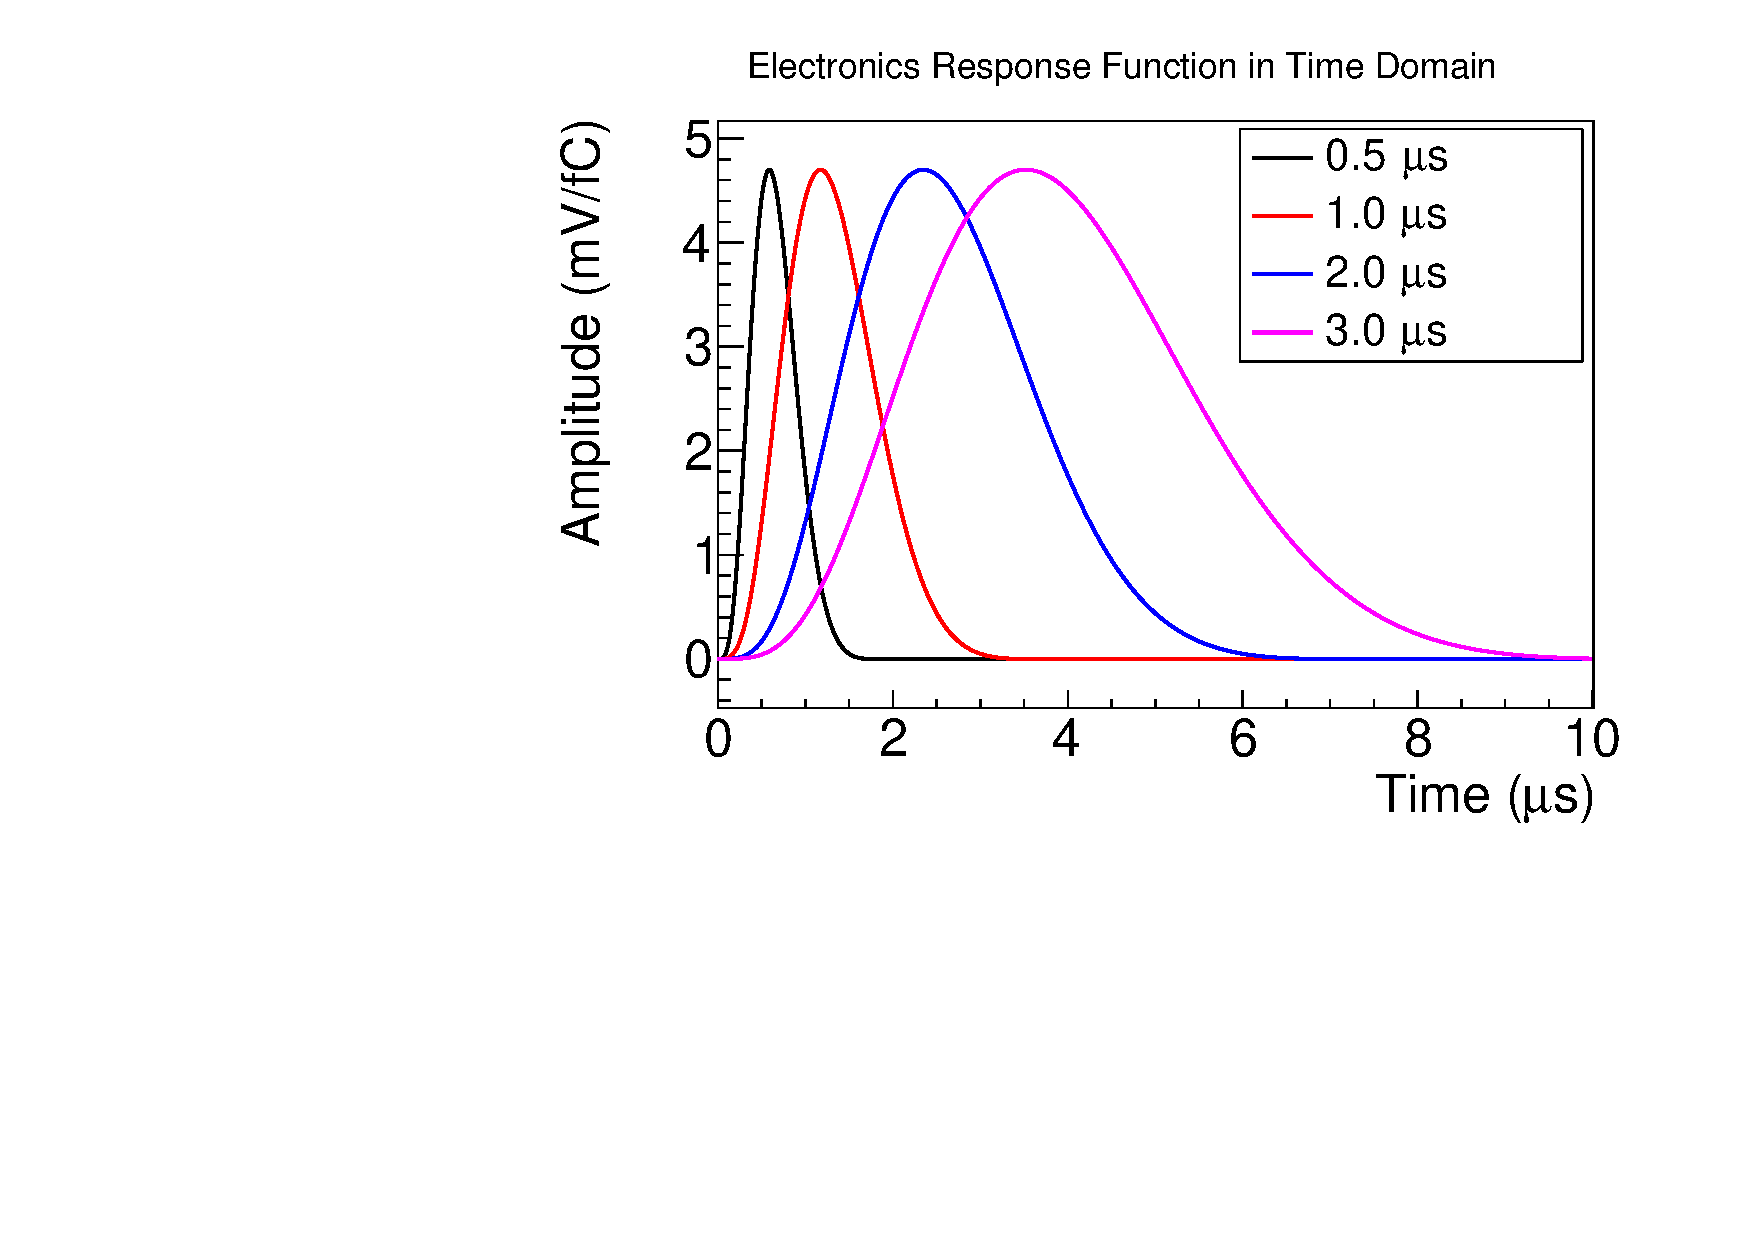
\includegraphics[width=0.6\textwidth]{electronics_res.pdf}
\end{cdrfigure}


While the principle is straightforward, calculating the measured
current itself can be very complicated. As shown in
Figure~\ref{fig:signal_formation}, the weighting field becomes smaller
at locations further away from the wire of interest.  
The weighting field also extends beyond the ``boundary'' of the wire.
Wire boundaries are defined by imaginary planes parallel to a wire,
perpendicular to the wire's plane and halfway between two neighboring
wires; i.e.,  in an ideal case, all charge produced within a wire's boundary
will drift to its nearest associated wire. 
%Due to the extent of 
Since a weighting field extends beyond a given wire's boundary, electrons drifting inside
this boundary can induce current in other wires.  
The induced currents therefore strongly depend on the local ionization
charge distribution near the wire of interest, which in turn depends
on the event topology of the initial energetic, charged particles.
%This fact makes the induced currents strongly depend on the local ionization charge distribution near the wire of interest, 


To illustrate the complication of the induction plane signal,  
an ideal track with a uniform charge distribution along it %the track 
is shown as 
an example in Figure~\ref{fig:ideal_track_1}. In the left panel, the 
two black lines represent the boundaries of one wire's region. In this case,  
%if one just counts 
counting only the ionization charge distribution within the wire's boundaries,
the expected 
distribution is shown in panel a) at top right.  However, the induced current on the wire of 
interest depends on the weighting field, which is smaller when the ionization electron is 
further away from the wire itself. Therefore, the effective charge distribution seen by 
the wire would be similar to what is shown in panel b) on the right side of 
Figure~\ref{fig:ideal_track_1}. 
\fixme{Why is signal in b) symmetric, when weighting potential for shown track is not ? - TK}
However, the wire of interest will experience an 
additional induced current from ionization electrons 
drifting outside its boundaries and in the regions of nearby wires. 
Since these ionization electrons are further away, 
the weighting field is even smaller and thus the induction from them is 
also smaller. A realistic effective charge distribution will be similar to the one shown in panel c) on 
the bottom right side of Figure~\ref{fig:ideal_track_1}. 


When the bipolar induction field response function is taken into account the 
charge transients change shape.
In the left panel of Figure~\ref{fig:ideal_track_2}, the top half shows 
the real charge distribution going through the targeted wire region. The convolution of this 
distribution with a bipolar response function will lead to results shown at the bottom. In this 
case, it can be seen that the signal height is still large at least for the start and the end of the 
signal. In the right panel of Figure~\ref{fig:ideal_track_2}, the top half shows the more 
realistic effective charge distribution seen by the targeted wire. The convolution of this 
distribution with a bipolar response function will lead to results shown at the bottom. In 
this case, it is apparent that the signal height is much smaller though the length of the signal is 
longer. This effect leads to complications in designing the data compression algorithm.

\begin{cdrfigure}[Induction plane field response for an ideal track (1)]{ideal_track_1}{Illustration of the induction plane field response for an ideal track (red arrow).}
  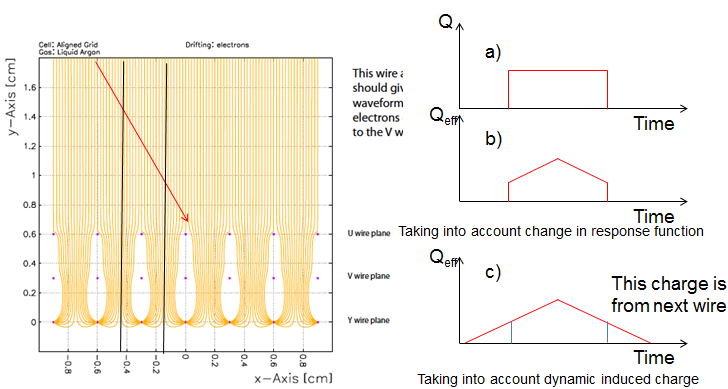
\includegraphics[width=0.7\textwidth]{ideal_track.png}
\end{cdrfigure}

\begin{cdrfigure}[Induction plane field response for an ideal track (2)]{ideal_track_2}{Illustration of the induction plane field response for an ideal track.}
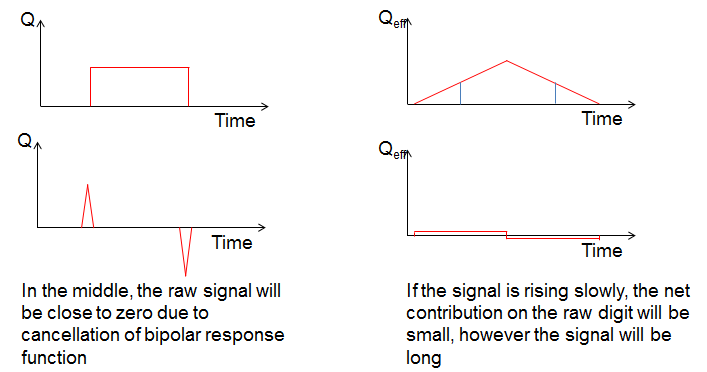
\includegraphics[width=0.75\textwidth]{ideal_track_2.png}
\end{cdrfigure}

%%%%%%%%%%%%%%%%%%%%%%%%%%%%%%%%%%%%%%%%%%%%%%
%%%%%%%%%%%%%%%%%%%%%%%%%%%%%%%%%%%%%%%%%%%%%%
\section{TPC Charge Extraction}
\label{sec:tpc-signal-calibration}

In Section~\ref{sec:tpc_signal_formation}, the signal formation in a single-phase LAr TPC
is described. This section describes the procedure of the TPC 
charge extraction. As shown in Figure~\ref{fig:signal_formation}, the 
goal of TPC charge extraction is to recover the number of ionized 
electrons from the digitized TPC signal. 

%%%%%%%%%%%%%%%%%%%%%%%%
\subsection{Deconvolution Technique}\label{sec:decon}
\label{sec:decon-tech}
Deconvolution is a mathematical technique to extract the \textit{underlying true signal}
$S(t)$ from a \textit{measured signal} $M(t_0)$. The deconvolution technique 
was introduced to LArTPC signal processing in LarSoft in the context of ArgoNEUT data analysis~\cite{bruce}. 
The goal of the deconvolution is 
to ``remove'' the field and electronics response functions from the measured 
signal to recover the underlying true number of ionizing electrons.~\footnote{Strictly speaking,
the deconvolution replaces the bipolar response function with a unipolar smearing
function.} This technique has the advantage of being robust and fast and is an 
essential step in the overall charge extraction process. 

The measured signal is modeled as a convolution integral over the true 
signal $S(t)$ and a given detector \textit{response function} $R(t,t_0)$ which gives the
instantaneous portion of the measured signal at some time $t_0$ due to
an element of the true signal at time $t$.
\begin{equation}\label{eq:decon_1}
M(t_0) = \int_{-\infty}^{\infty}  R(t,t_0) \cdot S(t) \cdot dt.
\end{equation}
If the detector response function only depends on the relative time 
difference between $t$ and $t_0$, the above equation can be solved by 
doing a Fourier transformation on both sides of the equation:
\begin{equation}
M(\omega) = R(\omega) \cdot S(\omega), 
\end{equation}
where $\omega$ is the frequency. In this case, we can derive the signal in the 
frequency domain by taking the ratio of the measured signal and the assumed
response function:
\begin{equation}\label{eq:decon_2}
S(\omega) = \frac{M(\omega)}{R(\omega)}.
\end{equation}
The true underlying signal in the time domain can then be obtained by applying the 
inverse Fourier transformation from the frequency domain. 

The Shockley-Ramo response function $R(\omega)$ does not address
contributions to the measured signal which are due to real world
sources of electrical \textit{noise} from thermal and unwanted transmitting
sources or due to the approximation in the digitization.
Such contributions to $M(\omega)$ will not be ``divided out'' by the deconvolution.
Worse, because the response function becomes small (see Section~\ref{sec:decon-2D-ind}) %below) 
at low 
frequencies for the induction planes and at high frequencies for all
planes, the noise components in these frequencies will become
enhanced by the deconvolution.

To address the problem of noise, a \textit{filter function} $F(\omega)$ is
introduced.  Its purpose is to attenuate the problematic noise.  The
addition of this function can be considered an augmentation to the
response function, which may in any case be chosen freely as it is a model.  
The two functions are kept distinct for clarity in the notation here.
Equation~\ref{eq:decon_2} is then updated to become
\begin{equation}\label{eq:decon_filt}
S(\omega) = \frac{M(\omega)}{R(\omega)} \cdot F(\omega).
\end{equation}
With a suitable noise model, an improved estimator for the signal
$S(t)$ in the time domain can then be found by applying an inverse Fourier 
transform to $S(\omega)$.  Essentially, the deconvolution replaces the field and 
electronics response function with the filter response function. The 
advantage of this procedure shows up on the induction plane where the irregular bipolar 
field response function is replaced by a regular unipolar response function through
the inclusion of the software filter. 


%%%%%%%%%%%%%%%%%%%%%%%%
\subsection{Importance of 2D Deconvolution for Induction Planes}
\label{sec:decon-2D-ind}

The 1D deconvolution procedure described in Section~\ref{sec:decon-tech} %the previous section 
works well in dealing with signal in the collection wire plane, but is not 
optimal when applied to signals in the induction wire planes. 
As described in Section~\ref{sec:tpc_signal_formation}, the induction plane wire 
signal receives contributions not only from ionization charge 
passing by the wire of interest, but also from ionization charge drifting in 
nearby wire boundaries. In addition, within the boundary of the wire of 
interest, the value of the field response function varies appreciably 
 so at small scales the location of the drifting charge relative to the wire 
is important. In this case, Equation~\ref{eq:decon_1} would naturally expand to 
\begin{equation}\label{eq:decon_2d_1}
M_i(t_0) = \int_{-\infty}^{\infty} \left( R_0 \cdot (t-t_0) \cdot S_i(t) + 
R_1 \cdot (t-t_0) \cdot S_{i+1} (t) + ...\right) \cdot dt,
\end{equation}
where $M_i$ represents the measured signal from wire $i$.  $S_i$ and
$S_{i+1}$ represents the true signal in the boundaries of wire $i$ and
its next neighbor, respectively.
$R_0$ represents the average response function for an ionization
charge passing through the region for the wire of interest.
Similarly, $R_1$ represents the average response function for an
ionization charge drifting through the next adjacent wire region. One can
easily expand this definition to some number of neighbors by introducing terms up 
to $R_{n-1}$.

If one applies a Fourier transformation on both sides of Equation~\ref{eq:decon_2d_1},
we have:
\begin{equation}\label{eq:decon_2d_2}
M_i(\omega) = R_0(\omega) \cdot S_i(\omega) + R_1(\omega) \cdot S_{i+1} (\omega) + ...,
\end{equation} 
which can be written in a matrix notation as:
\begin{equation}
\begin{pmatrix}
    M_1(\omega)\\
    M_2(\omega)\\
    \vdots\\
    M_{n-1}(\omega)\\
    M_{n}(\omega)
\end{pmatrix}
=
\begin{pmatrix}
R_0(\omega) & R_1(\omega) & \ldots & R_{n-2}(\omega) & R_{n-1}(\omega) \\
R_1(\omega) & R_0(\omega) & \ldots & R_{n-3}(\omega) & R_{n-2}(\omega) \\
    \vdots  & \vdots      & \ddots & \vdots          & \vdots \\
    R_{n-2}(\omega) & R_{n-3}(\omega) & \ldots & R_0(\omega) & R_1(\omega) \\
    R_{n-1}(\omega) & R_{n-2}(\omega) & \ldots & R_1(\omega) & R_0(\omega) \\
\end{pmatrix}
\cdot
\begin{pmatrix}
    S_1(\omega)\\
    S_2(\omega)\\
    \vdots\\
    S_{n-1}(\omega)\\
    S_{n}(\omega)
\end{pmatrix}
\label{eq:matrix_expansion}
\end{equation}
Assuming the response functions (i.e., the matrix $R$) are known, the 
problem converts into deducing the vector of $S$ with the measured signal $M$. 
%
This can be achieved by inverting the matrix $R$. In practice and away
from plane edges the matrix $R$ is taken to be symmetric and its
inversion can again be achieved by FFT.
%
As this expands the 1D deconvolution (with respect to the time axis)
into a 2D deconvolution (with respect to both the time and wire
axes), the filter function must be expanded in a similar fashion to cover
both time and wire dimensions.

A comment on the limitation (or approximation) 
assumed in the 2D deconvolution is needed. As shown in Equation~\ref{eq:decon_2d_1}, the 
average response functions are used in describing the measured signal. These 
ignore the detailed position dependence of the response function. 
This approximation ignores the fine-grained but clear position
dependence in the calculated weighting fields.
However, since the signal from any given wire can only be measured as
a function of time, there is no additional information to be used to
resolve the ionization electron distributions within a wire boundary.
This technique can in principle be improved to include the position-dependent
response once the local ionization charge distribution is roughly reconstructed. 

%%%%%%%%%%%%%%%%%%%%%%%%
\subsection{Additional Challenges in Deconvolution}


The 1D and 2D deconvolution procedures provide a robust method to extract the ionization
electrons for the collection and induction planes, respectively. 
%
While working well for the collection plane, the procedure is still not optimal 
for the induction plane due to the nature of the induction plane signal. 
Figure~\ref{fig:induction_field} shows the field response as simulated with Garfield~\cite{garfield}
for induction and collection wire planes and point ionization
electrons. While the field response for the collection wire plane is unipolar, the field 
response for the induction wire plane is bipolar. 
%
\begin{cdrfigure}[Simulated field response functions in the time and frequency domains]{induction_field}{(left) Simulated field response functions for induction (black and red) and 
collection (blue) wires are shown in the time domain. (right) The same are shown in 
the frequency domain.}
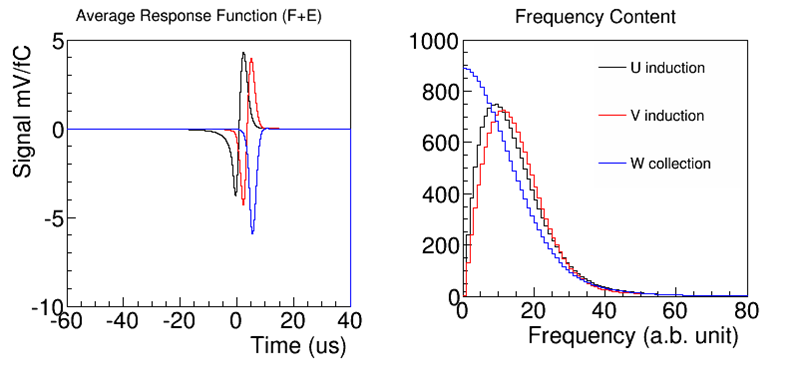
\includegraphics[width=0.95\textwidth]{induction_field_response.png}
\end{cdrfigure}
%
The early, negative half corresponds to the ionization electron moving
towards the wire plane and the late, positive half corresponds
to the ionization electron moving away.
%
The integration of the field response function is close to zero
as the bias wire voltages are applied such that that none of the ionization electrons are
collected. The right panel of Figure~\ref{fig:induction_field} shows the 
frequency components of the field response. 
%
Since an induction plane field response has a bipolar shape in the time domain 
there is a corresponding suppression at low frequency in the frequency 
domain. At zero frequency, the frequency component essentially gives the 
integration of field response function over time and thus should be near 
zero (again, because no charge is collected).


The suppression of the induction field response at low frequency is problematic for the
proposed deconvolution procedure. First,  the measured signal contains the electronic noise, 
which usually increases at low frequency (the so-called 1/f noise). Therefore, as shown in 
Equation~\eqref{eq:decon_filt}, the low-frequency noise will be amplified in the deconvolution 
process, since the denominator (i.e., the induction field response) is generally small at 
low frequency. This can be seen clearly in Figure~\ref{fig:decon_example}, where the low-frequency noise
is significant. The large low-frequency noise would lead to large uncertainty 
in the charge estimation, and needs to be dealt with.  

\begin{cdrfigure}[Example of deconvoluted spectrum for the induction plane (simulation)]{decon_example}{Example of deconvoluted spectrum for the induction plane (simulation).}
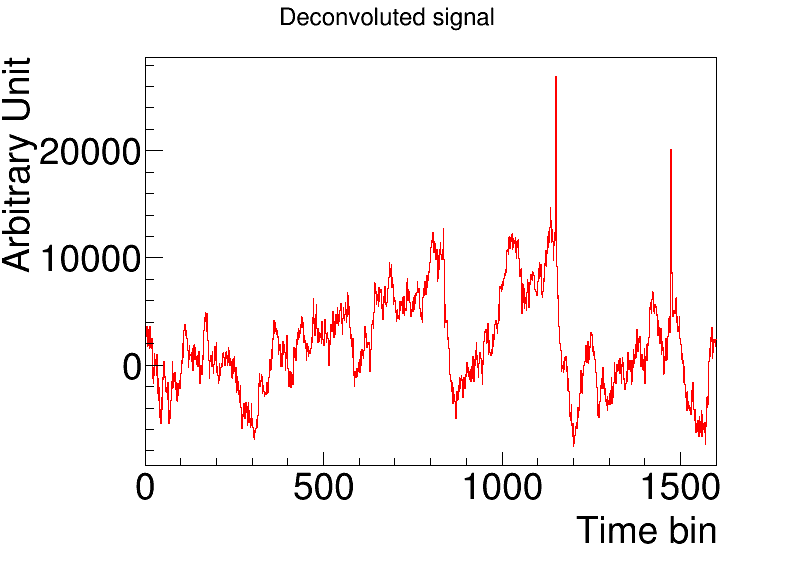
\includegraphics[width=0.6\textwidth]{decon_example.png}
\end{cdrfigure}


In Equation~\eqref{eq:decon_filt}, a frequency-domain  filter function is introduced 
to suppress the numerical instability caused by the presence of noise. One can imagine using % to use 
this software filter to suppress the electronic noise at low frequency. 
However, such a filter is not acceptable due to the large distortion which it introduces to the signal.
To illustrate this point, recall that the software filter is effectively a smearing function. 
Figure~\ref{fig:low_f_filter} shows an illustrative true signal (left), its convolution 
with a low-frequency filter (middle), and the low-frequency filter itself (right). 
It is obvious that the signal is strongly distorted due to the application of the 
low-frequency software filter. 

\begin{cdrfigure}[Impact of the low-frequency filter]{low_f_filter}{The impact of the low-frequency filter (right). The unit of the $x$-axis 
is MHz.  The true signal and the convoluted signal are shown in the left and
middle panels, respectively. A time tick corresponds to 0.5 $\mu s$.}
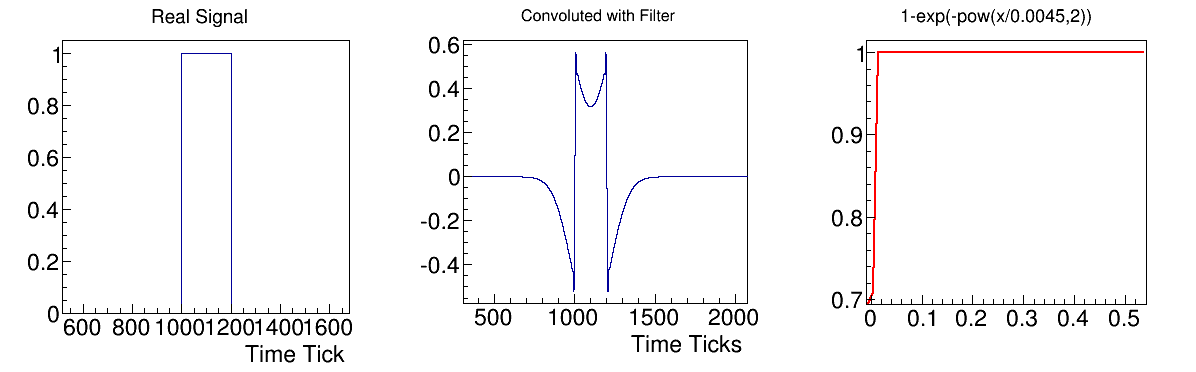
\includegraphics[width=0.95\textwidth]{low_freq.png}
\end{cdrfigure}

In order to deal with this problem, we turn to using two techniques in the time domain: 
\textit{region of interest (ROI)} and \textit{adaptive baseline (AB)}. The ROI technique~\cite{roi}
was proposed in the context of reducing data size and speeding up the 
deconvolution process. At the same time, the ROI technique can %also 
be used to 
suppress the low-frequency noise. In order to recognize this point, consider
a time window with $N$ time ticks.  For ProtoDUNE-SP, this would be a window of 
$N\times0.5\mu\mbox{s}$. The highest frequency that can be resolved with such 
sampling would be 1~MHz. The first discrete frequency above zero would be $2/N$ MHz, 
and no result within the ROI can be sensitive to any noise components below this 
frequency.  Therefore, if we can identify the signal region and create a ROI to 
cover the signal, we can naturally suppress the low-frequency noises. 

The adaptive baseline (AB) technique~\cite{ab} was introduced  
in the context of 
dealing with the ASIC saturation observed in MicroBooNE. The AB is essentially a 
local baseline calculated in a given a ROI. However, instead of a simple average of 
the baseline at the start and end points of a ROI, a linear interpolation is used to 
correct the baseline. Given the two constraints (start and end points of the ROI), 
the linear interpolation with two degrees of freedom is the best that one can achieve 
to remove bias in the baseline. 

In Section~\ref{sec:decon-frf-calc} %the following, 
we describe various techniques 
used in the charge extraction.

%%%%%%%%%%%%%%%%%%%%%%%%
\subsection{Calculation of Field Response Function}
\label{sec:decon-frf-calc}

The field response is calculated with Garfield~\cite{garfield} in a 22-cm (along the 
field direction) $\times$ 30-cm (along the wire plane direction) region in 2D.  
In the drift direction, the grid plane is labeled as G, the two induction %planes 
wire 
planes are labeled U and V, and the collection plane is W.  The spacing between the wire 
planes is 4.76~mm. The bias voltages of-665 V, -370 V, 0 V, and +820 V for the G, U, V, and 
W planes, respectively, are configured according the operating conditions that ensure 100\%
    transmission of ionization electrons through the first two induction planes.  
    101 wires of diameter 150 $\mu$m are set on each wire plane with a pitch of 4.667 (4.79 for collection) mm.  A ground plane is placed 1~cm behind the W plane.  The drift
    field is uniform with 500~V/cm. The electron drift velocity as a function of
    electric field is taken from measurements~\cite{Li:2015rqa,lar_property}
    instead of using the default velocity table contained in~\cite{garfield}. % Garfield. 
    The electron
    diffusion is turned off in the simulation. The field response function then can
    be calculated for each individual wire in the form of induction current 
    (U and V planes) and collection current on (W planes) as a function of time for
    an electron drift which starts from arbitrary position within the region of calculation. 
    \fixme{please clarify previous sentence. Here is my attempt to make it less of a mouthful: For an 
    electron drift that starts from an arbitrary position within the ROI, the field response then can
    be calculated for each individual wire in the form of induction current 
    (U and V planes) or collection current (W plane) as a function of time.}
    
    
    Figure~\ref{fig:garfield_2d} shows the configuration used in Garfield 2D simulation.
The Garfield-simulated response functions are shown in Figure~\ref{figs:overall_response}.
 The average response function for single electrons within a wire region 
is calculated for the closest wire $R_0$, next adjacent wire $R_1$, and so on. The U and 
V plane response functions are shown in the middle and right panel of 
Figure~\ref{figs:overall_response}, respectively.  For induction wire planes, these response 
functions are reasonably balanced, as expected.


\begin{cdrfigure}[Description of the Garfield 2D simulation of field response 
functions]{garfield_2d}{Description of the Garfield 2D simulation of field response functions}
  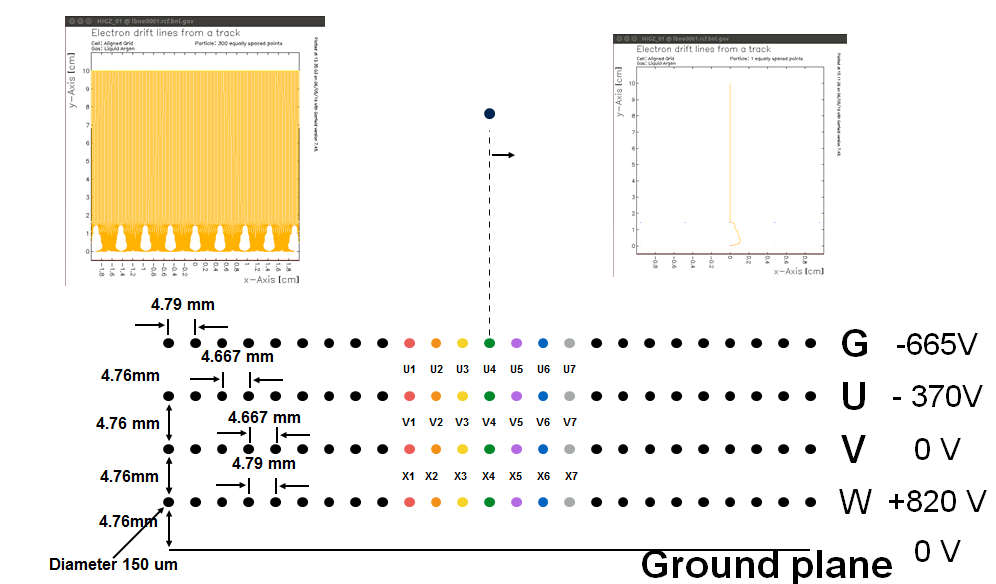
\includegraphics[width=0.95\textwidth]{Garfield_simu.png}
\end{cdrfigure}
\fixme{Figure~\ref{fig:garfield_2d} needs a more descriptive caption}


\begin{cdrfigure}[Overall response functions]{overall_response}{The overall response functions, i.e., %which is 
the convolution of the
electronics response function (14 mV/fC gain and 2 $\mu$s shaping time) 
and the field response.}
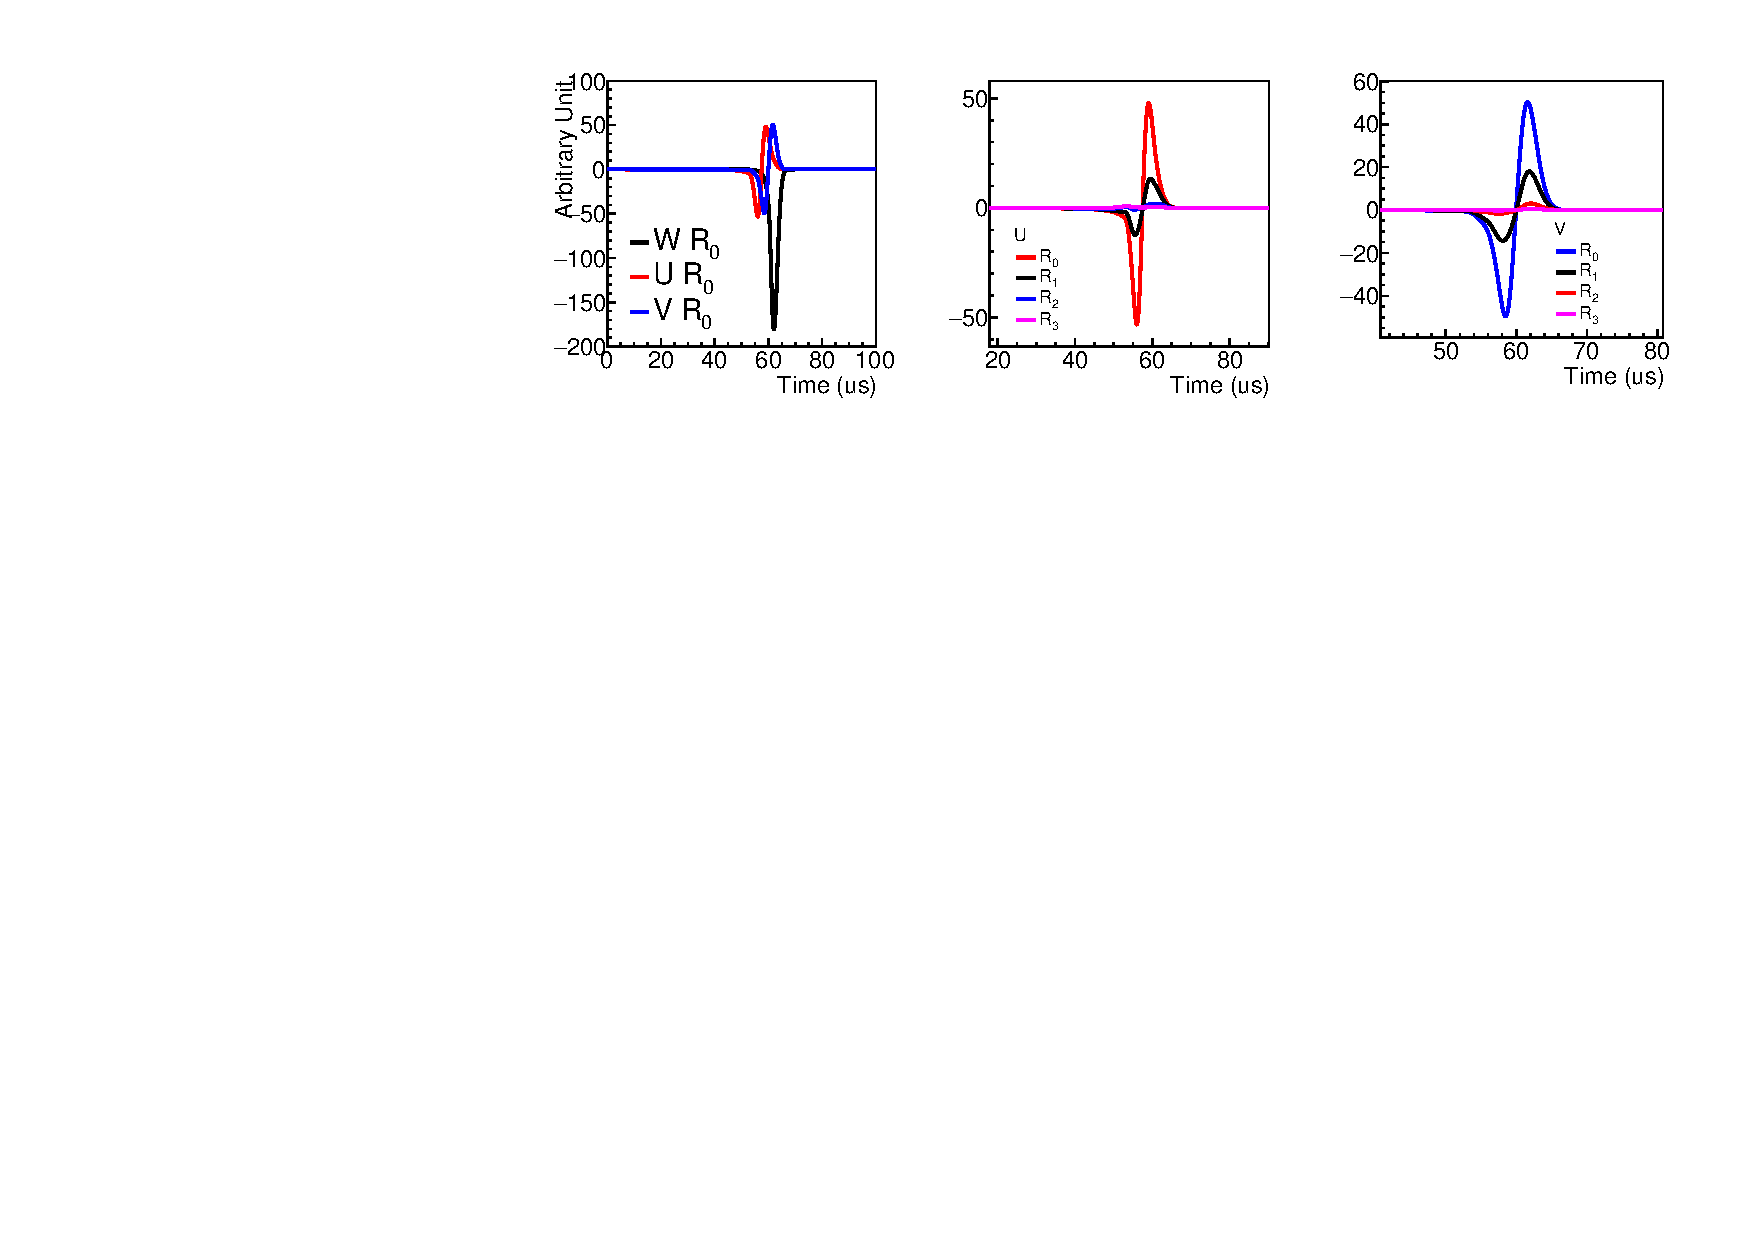
\includegraphics[width=0.95\textwidth]{dune_field_res.pdf}
\end{cdrfigure}
\fixme{This could use more description, but I guess it's clear what each panel is}

%%%%%%%%%%%%%%%%%%%%%%%%
\subsection{Choice of Software Filter}

Two types of filters are selected and implemented.  The first, inspired by the Wiener filter,  
 is modified to not suppress low-frequency components.  The second is the 
Gaussian filter. While the first one is optimized \fixme{independently?} for each wire plane to produce a 
high signal-to-noise ratio, the second one is optimized for the three planes as a group % and same to all the planes 
to correctly estimate the charge which is independently measured on each  plane. %of the three planes.  
This latter is important if all three planes are used for energy measurement 
and is critical for proper application of the Wire-Cell imaging technique~\cite{wire-cell}.  
In this section, we describe the selection process that resulted in %choice on 
these software filters.

The standard Wiener noise filter~\cite{wiener} is constructed using the expected 
signal $S(\omega)$ and noise $N(\omega)$ frequency spectra:
\begin{equation}
F(\omega) = \frac{S^2(\omega)}{S^2(\omega) + N^2(\omega)}.
\end{equation}
With this construction, the Wiener filter is expected to achieve the best signal-to-noise ratio. 
However, applying the Wiener filter to TPC signal processing is problematic. 
First, in a LArTPC, the TPC signal $S(\omega)$ varies substantially
depending on the exact nature of the event topology.
Second, the electronic noise spectrum is a function of the time window
over which it is observed. A longer time window allows for observation
of more low-frequency noise components.
Third, the induction wire signal spectrum is small at low frequency
and so would be its \fixme{own?} Wiener filter.  However, as discussed previously, 
a software filter with low-frequency suppression leads to large distortions 
of the signal and is thus not ideal.  

The functional form of the software filter is chosen as:
\begin{equation}
F(\omega) = 
\begin{cases}
e^{- \frac{1}{2} \cdot \left( \frac{\omega}{a} \right)^b} &  \omega >0 \\
0 &  \omega = 0, \\
\end{cases}
\end{equation}
where $a$ and $b$ are two free parameters.  Note, $b=2$ is basically the Gaussian filter. 
The filter is explicitly zero at $\omega = 0$ in order to remove the DC component in the 
deconvoluted signal. This removes information about the baseline;  a new baseline is 
calculated and restored for the waveform after deconvolution. The above functional form 
of the filter has another advantageous property:
\begin{equation}
lim_{\omega \rightarrow 0} F(\omega) = 1.
\end{equation}
which means the integral of the smearing function is unity, which does not introduce any
extra factor in the overall normalization. The free parameters $a$ and $b$ in the above 
form are determined by matching the tail of Wiener filter at its high-frequency side. 
An example of a software filter is shown in Figure~\ref{fig:soft_filter_1}. 

\begin{cdrfigure}[Wiener-inspired filter and Gaussian filter used in the 2D deconvolution]{soft_filter_1}{The Wiener-inspired filter and Gaussian filter used in the 2D deconvolution. 
The time and frequency domain content are shown on the left and right panel, respectively.
The x-axis's unit for the time domain is $\mu$s. For the frequency domain, the number 2000
corresponds to $\sim$0.42 MHz.}
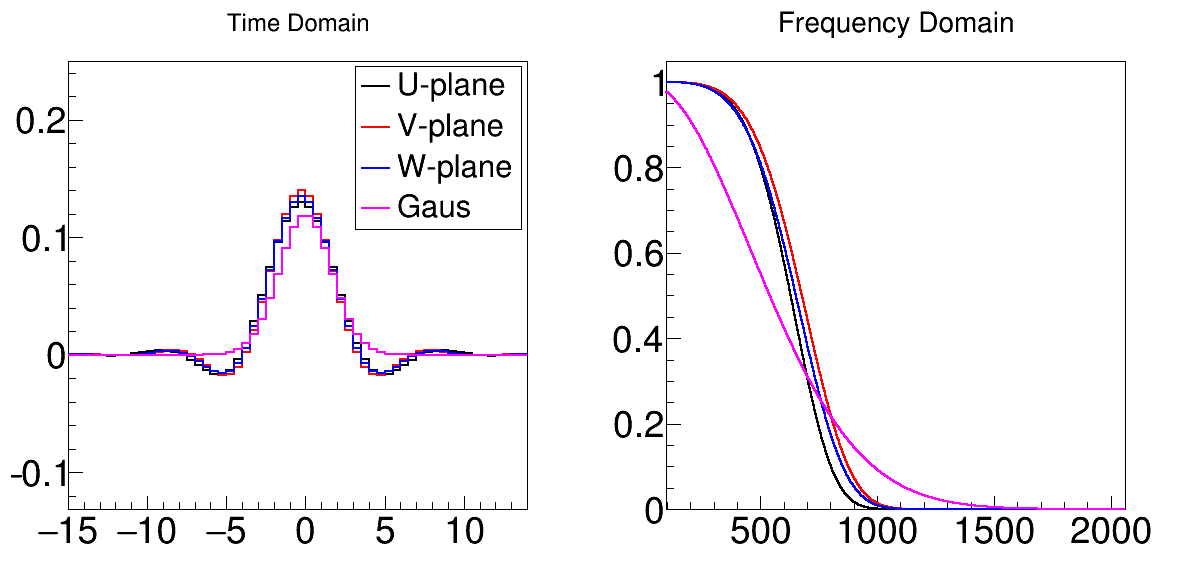
\includegraphics[width=0.8\textwidth]{filter_1.png}
\end{cdrfigure}

Beside the high-frequency software filter described above, there is also a low-frequency 
software filter which is used to select ROIs (discussed in Section~\ref{sec:decon-roi-selection}.) %the next section). 
The functional form of the low-frequency software filter is chosen to be 
\begin{equation}
F(\omega) = 1- e^{-\frac{1}{2}\cdot \left( \frac{\omega}{c} \right)^2}.
\end{equation}

%%%%%%%%%%%%%%%%%%%%%%%%
\subsection{ROI Selection}
\label{sec:decon-roi-selection}

The region of interest (ROI) is an important technique for limiting the contribution of low-frequency 
electronic noise. The ROI selection was based on the deconvoluted results. Essentially, we perform
two rounds of deconvolution:
\begin{itemize}
\item 2D deconvolution with the balanced Garfield-simulated field response function with a low-frequency filter (``2D deconvolution with low-frequency filter'').
\item 2D deconvolution with the balanced Garfield-simulated field response function without a low-frequency filter (``2D deconvolution'').
\end{itemize}
The first one is used to select ROIs, and the results from the second deconvolution are then 
used to obtain the final deconvoluted results. 

%%%%%%%%%%%%%%%%%%%%%%%%
\subsection{Metrics in Evaluating TPC Signal Processing}

In order to evaluate the TPC signal processing, which includes both the noise filtering and 
the charge extraction, two robust metrics can be used. % for evaluation purpose. 
They are:
\begin{itemize}
\item Equivalent Noise Charge (ENC): \\
  ENC is  basically proportional to the pedestal RMS in terms of ADC, and is a direct 
measure of the noise level in %the unit of 
electrons. It can be used to compare the 
noise levels from different experiments.
\item Deconvoluted Noise Charge after the TPC charge extraction (DNC): \\
The goal of the TPC charge extraction process is to recover the number of ionization 
electrons from the measured TPC signal. With the same procedure, the electronic noise
will also be converted. %The unit of these noise is again 
This is again measured in electrons, %which 
and so can be compared with 
the expected ionization electrons from energetic charged particles. 
The DNC depends on the ENC and on the frequency content of the noise spectrum. It also depends 
on the response function used for deconvolution, which is the primary reason 
why the induction plane DNC is much higher than the collection plane DNC. Furthermore, since
we have to rely on ROI and AB techniques to reduce the noise level for the induction plane, the
DNC also depends on the time-window length of the ROI. 
\end{itemize}
Understanding the ENC and DNC for the current-generation experiments and the expected 
performance for the future experiments are important steps to achieve automated event 
reconstruction for LArTPCs.

\begin{cdrfigure}[Residual noise vs wire length]{rms3}{The noise level in terms of the RMS value and ENC 
is plotted with respect to the wire length observed in MicroBooNE. 
This plot is taken from~\cite{noise_filter}.}
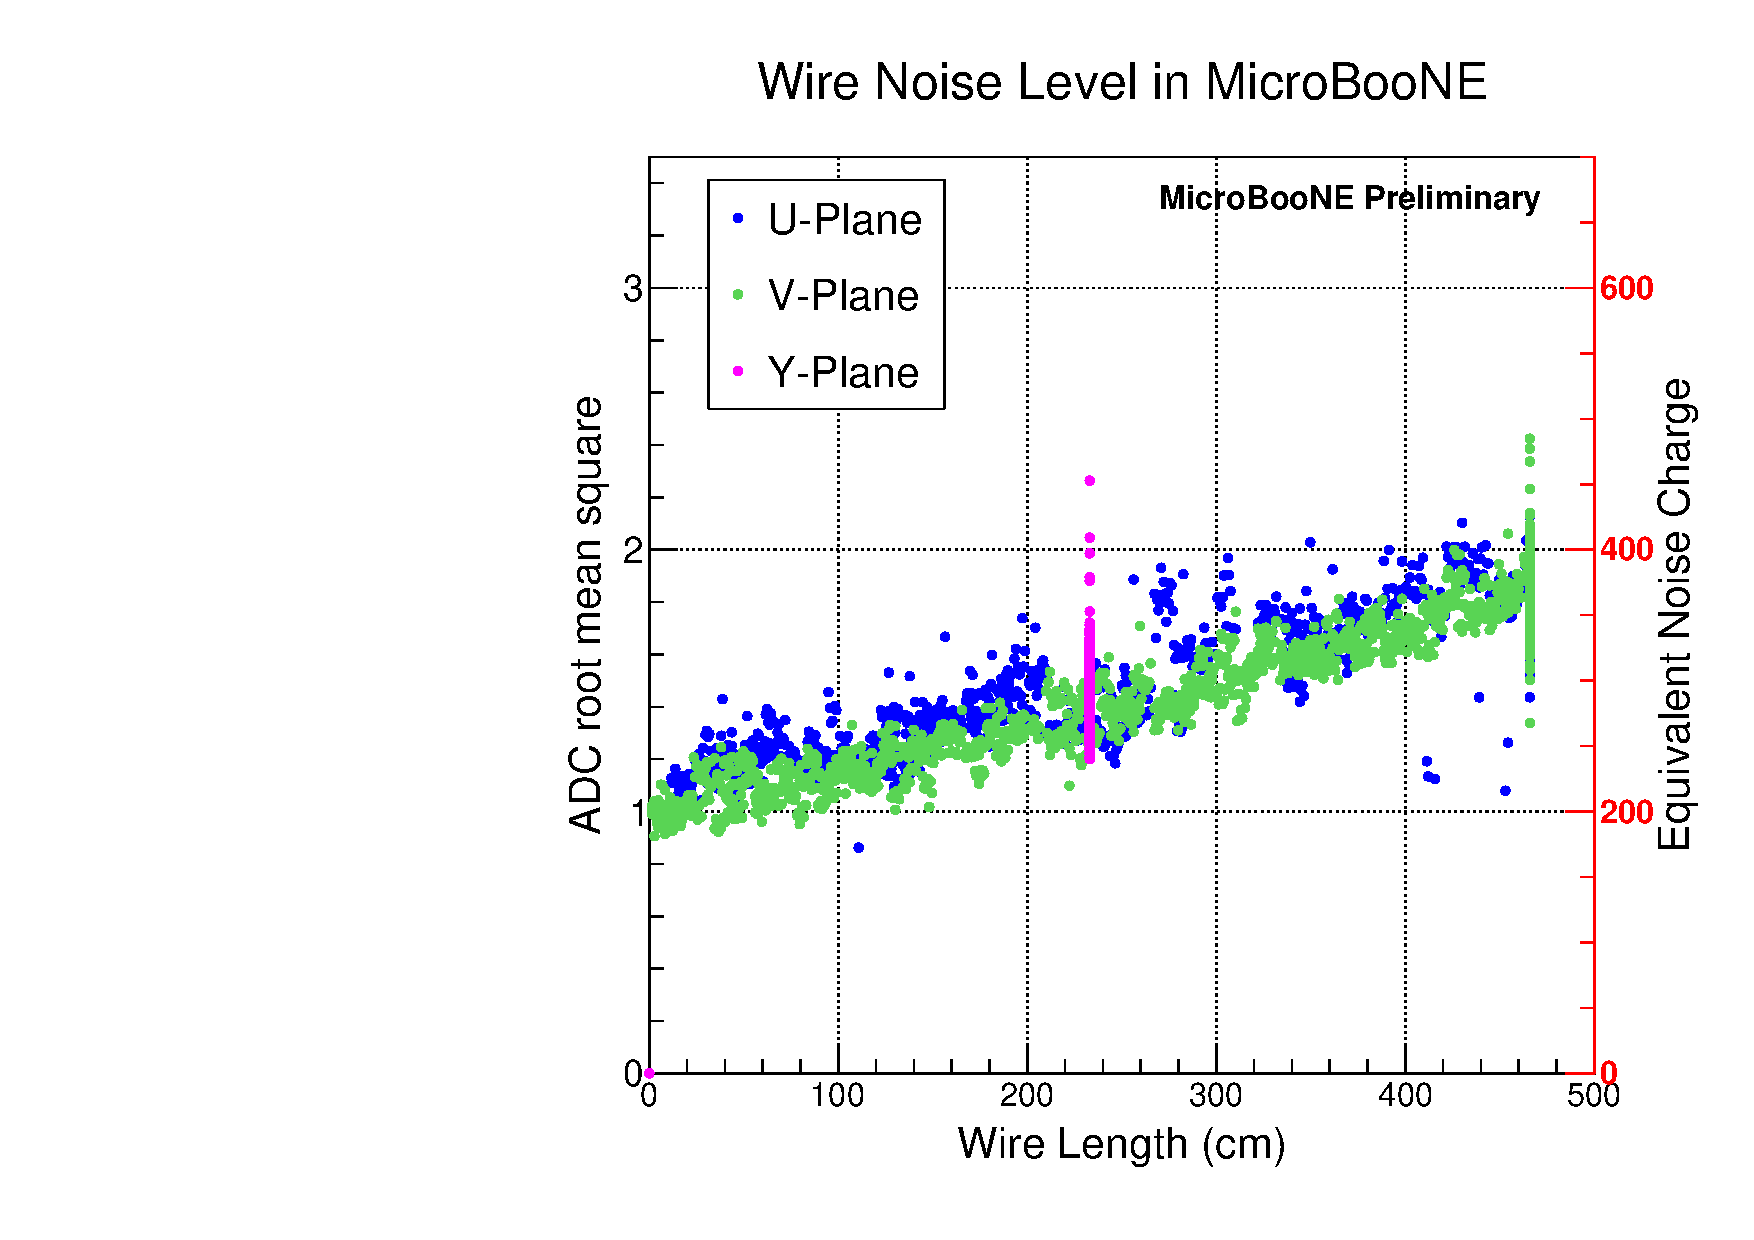
\includegraphics[width=0.75\textwidth]{RMSvsLength_after.pdf}
\end{cdrfigure}

The ENC in MicroBooNE has been reported at~\cite{noise_filter} and plotted 
in Figure~\ref{rms3}. As illustrate above \fixme{reference section or figure}, the calculation of the DNC depends on the 
drifted-charge extraction procedure. More specifically, it depends on the field 
response, the noise level (ENC and the frequency content), and the length of the ROI. 
Figure~\ref{DNC} shows the calculated DNC as a function of the time-window length 
for the second induction (V) plane, which is expected to have the smallest field 
response function (thus the largest DNC). 

\begin{cdrfigure}[Calculation of DNC vs time window length for second induction (V) plane]{DNC}{Calculation of DNC with respect to the time window length for second induction (V) plane. 
The ENC used in this simulation is 500 electrons given the induction wire length in protoDUNE. 
The red line shows the expected signal size for a minimal ionizing particle (MIP) 
traveling 3.2 mm.}
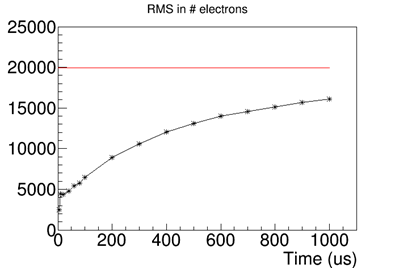
\includegraphics[width=0.75\textwidth]{DNC.png}
\end{cdrfigure}




%   It is:    \section{TPC Charge Extraction}


%%%%%%%%%%%%%%%%%%%%%%%%%%%%%%%%%%%%%%%%%%%%%%
\section{Space charge effect}

%%%%%%%%%%%%%%%%%%%%%%%%
\subsection{Introduction} \label{sec:SCEintro}

In order to correctly reconstruct the trajectories of particles that travel through the active volume of the TPC as well as precisely determine calorimetric information for these particles, it is essential to know very well the magnitude and direction of the drift electric field throughout the TPC bulk.  Nominally the electric field should be uniform throughout the TPC volume.  However, field effects such as the space charge effect (SCE) may cause distortions in the electric field that result in distortions in the reconstructed position of ionization electron clusters detected by the TPC wire planes as well as variation in the relative level of electron-ion recombination in different parts of the TPC~\cite{KirkSCE}.  The space charge effect is the build-up of slow-moving positive ions in a detector due to, for instance, ionization from cosmic muons.  As ProtoDUNE-SP is a detector on the surface with little overburden, the cosmic muon flux is expected to create a significant amount of space charge (positive argon ions) that could modestly impact the drift electric field within the TPC active volume.

In principle this effect could have modest impact in any TPC (liquid or gaseous) if the dimensions of the detector -- in particular the maximal drift distance -- are large enough to accumulate a high ion density.  In these cases, having a robust calibration method is necessary in order to account for the effect in particle trajectory reconstruction and calorimetry.  An example of the impact of the space charge effect on track reconstruction is shown in Figure~\ref{fig:SCEtrackEffects}~\cite{Mooney:2015kke}.  It should be understood that observations of these spatial distortions in data may include other effects, e.g., distortions of the applied field due to geometric and electric potential errors, distortion of the wire geometry, etc.  Within the context of this section, these other possible sources of distortions in reconstructed ionization electron cluster position are ignored as they are expected to be small in comparison with the distortions caused by the SCE.

\begin{cdrfigure}[Impact of the space charge effect on reconstructed tracks in the detector.]{SCEtrackEffects}{Impact of the space charge effect on reconstructed tracks in the detector.  The impact on a reconstructed track can be broken up into two distinct features:  a squeezing of the sides of the tracks in the transverse TPC directions that can somewhat resemble a rotation (``A'') and a bowing of the track toward the cathode that is most pronounced in the middle of the TPC (``B'').}
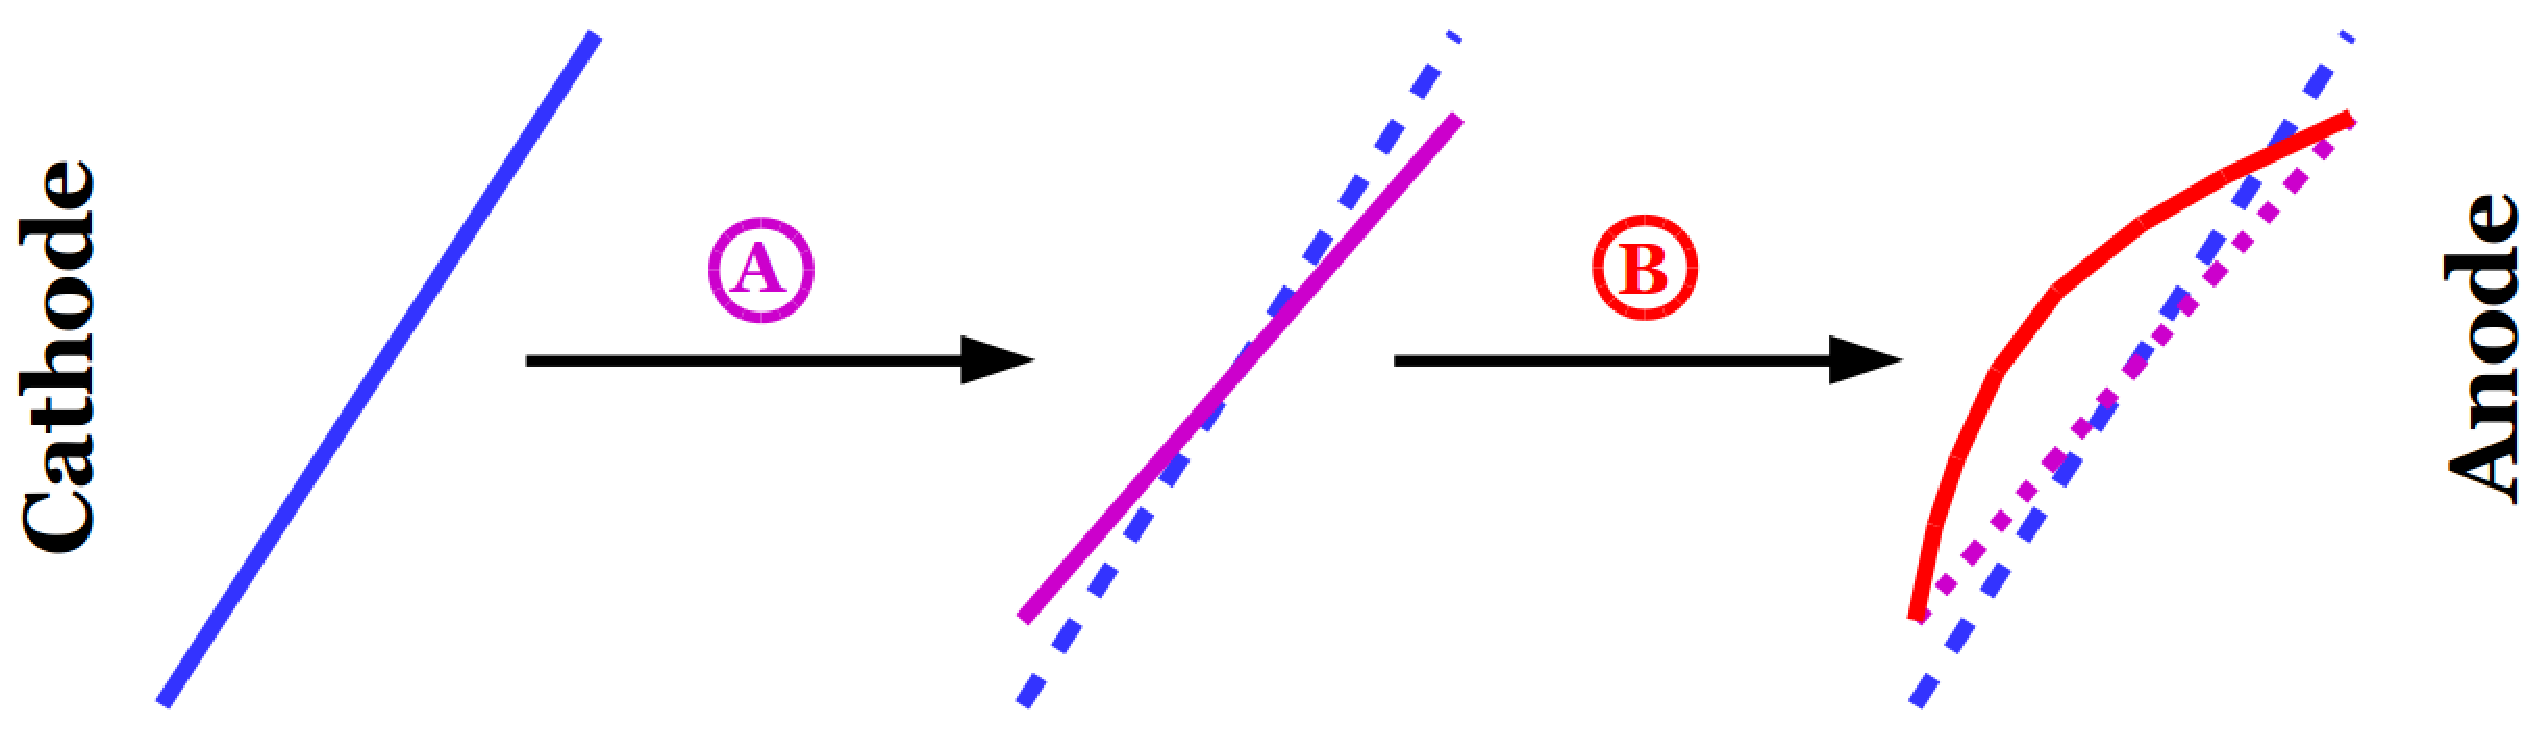
\includegraphics[width=0.99\linewidth]{trackSCE.pdf}
\end{cdrfigure}


%%%%%%%%%%%%%%%%%%%%%%%%
\subsection{Simulation} \label{sec:SCEsim}

Software was developed~\cite{SCEsimNote} to simulate the impact of space charge on the electric field within the TPC, along with the distortions in reconstructed ionization electron position at different points within the TPC bulk.  This simulation makes use of a Fourier series solution to the boundary value problem to solve for the electric field on a three-dimensional grid within the bulk of the TPC, an interpolation in between the grid points using radial basis functions to find the electric field everywhere in the TPC, and ray-tracing using the RKF45\footnote{``Runge–Kutta–Fehlberg 4(5)'' method, an algorithm for the numerical solution of ordinary differential equations.} method in order to simulate the distortions in reconstructed position of ionization electron clusters.

An assumption is made that the charge deposition rate from cosmic muons is uniform across the TPC volume:  $2{\times}10^{-10}~\mathrm{C}/\mathrm{m}^{3}/\mathrm{s}$ at a drift field of 500~V/cm~\cite{KirkSCE}.  As a result, ignoring higher-order effects of the electric field distortions on the space charge configuration itself, the space charge density is linear with respect to the distance from the anode plane.  The space charge density profile used in the simulation is shown in Figure~\ref{fig:simSCDist} for a drift field of 500~V/cm.

\begin{cdrfigure}[Space charge density $\rho$ as a function of the $x$ position assumed in the simulation]{simSCDist}{Space charge density $\rho$ as a function of the $x$ position assumed in the simulation. The space charge density at the cathode, $90$ $\mathrm{nC}/\mathrm{m}^3$, reflects both the expected rate of cosmic ray charge deposition and effects of recombination~\cite{KirkSCE}. The distribution is independent of $y$ and $z$ in the simulation (an approximation).}
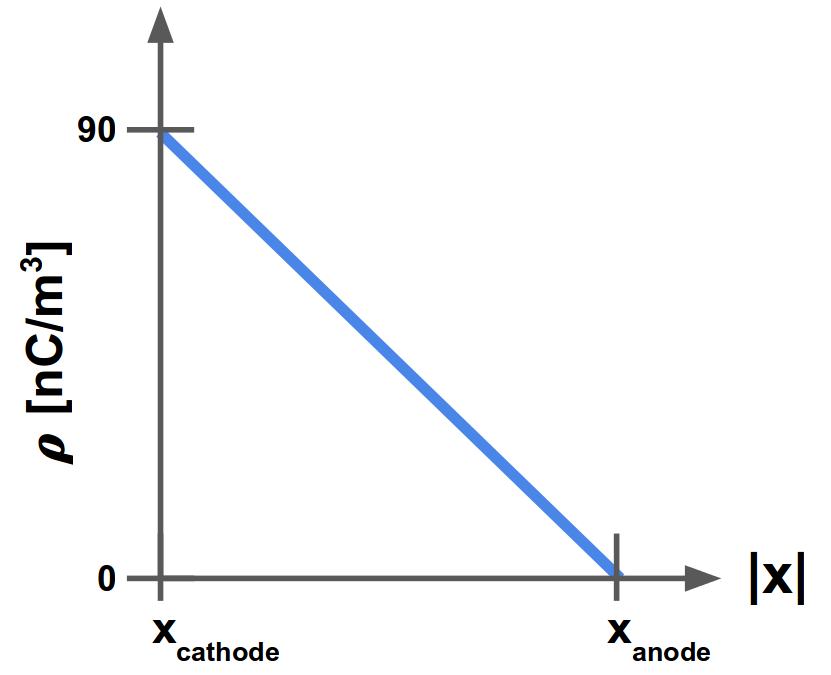
\includegraphics[width=.6\textwidth]{SCprofile.png}
\end{cdrfigure}


Some of the simulation results are shown in Figure~\ref{fig:simexample_Evals} and Figure~\ref{fig:simexample_Dvals}, which illustrate the impact of space charge on both the drift electric field (Figure~\ref{fig:simexample_Evals}) as well as the distortions in reconstructed ionization electron cluster position (Figure~\ref{fig:simexample_Dvals}).  At a drift field of 500~V/cm (corresponding to expected conditions during data-taking at protoDUNE), the expected maximal impact on the electric field is roughly 10\% in both the drift and transverse directions.

\begin{cdrfigure}[Simulated effects of space charge on the drift electric field in the ProtoDUNE-SP TPC]{simexample_Evals}{Illustration of the simulated effects of space charge on the drift electric field in the ProtoDUNE-SP TPC.  Results are shown for the effect in $x$ (top row), $y$ (middle row), and $z$ (bottom row).  The electric field distortions are normalized to the nominal drift electric field magnitude ($E_{0}$) of 500~V/cm and are plotted as a function of the true position in the TPC.  Simulation results are shown both for a central slice in $z$ (left column) and for a slice in $z$ closer to the end of the TPC, $z$ = 19 cm (right column).}
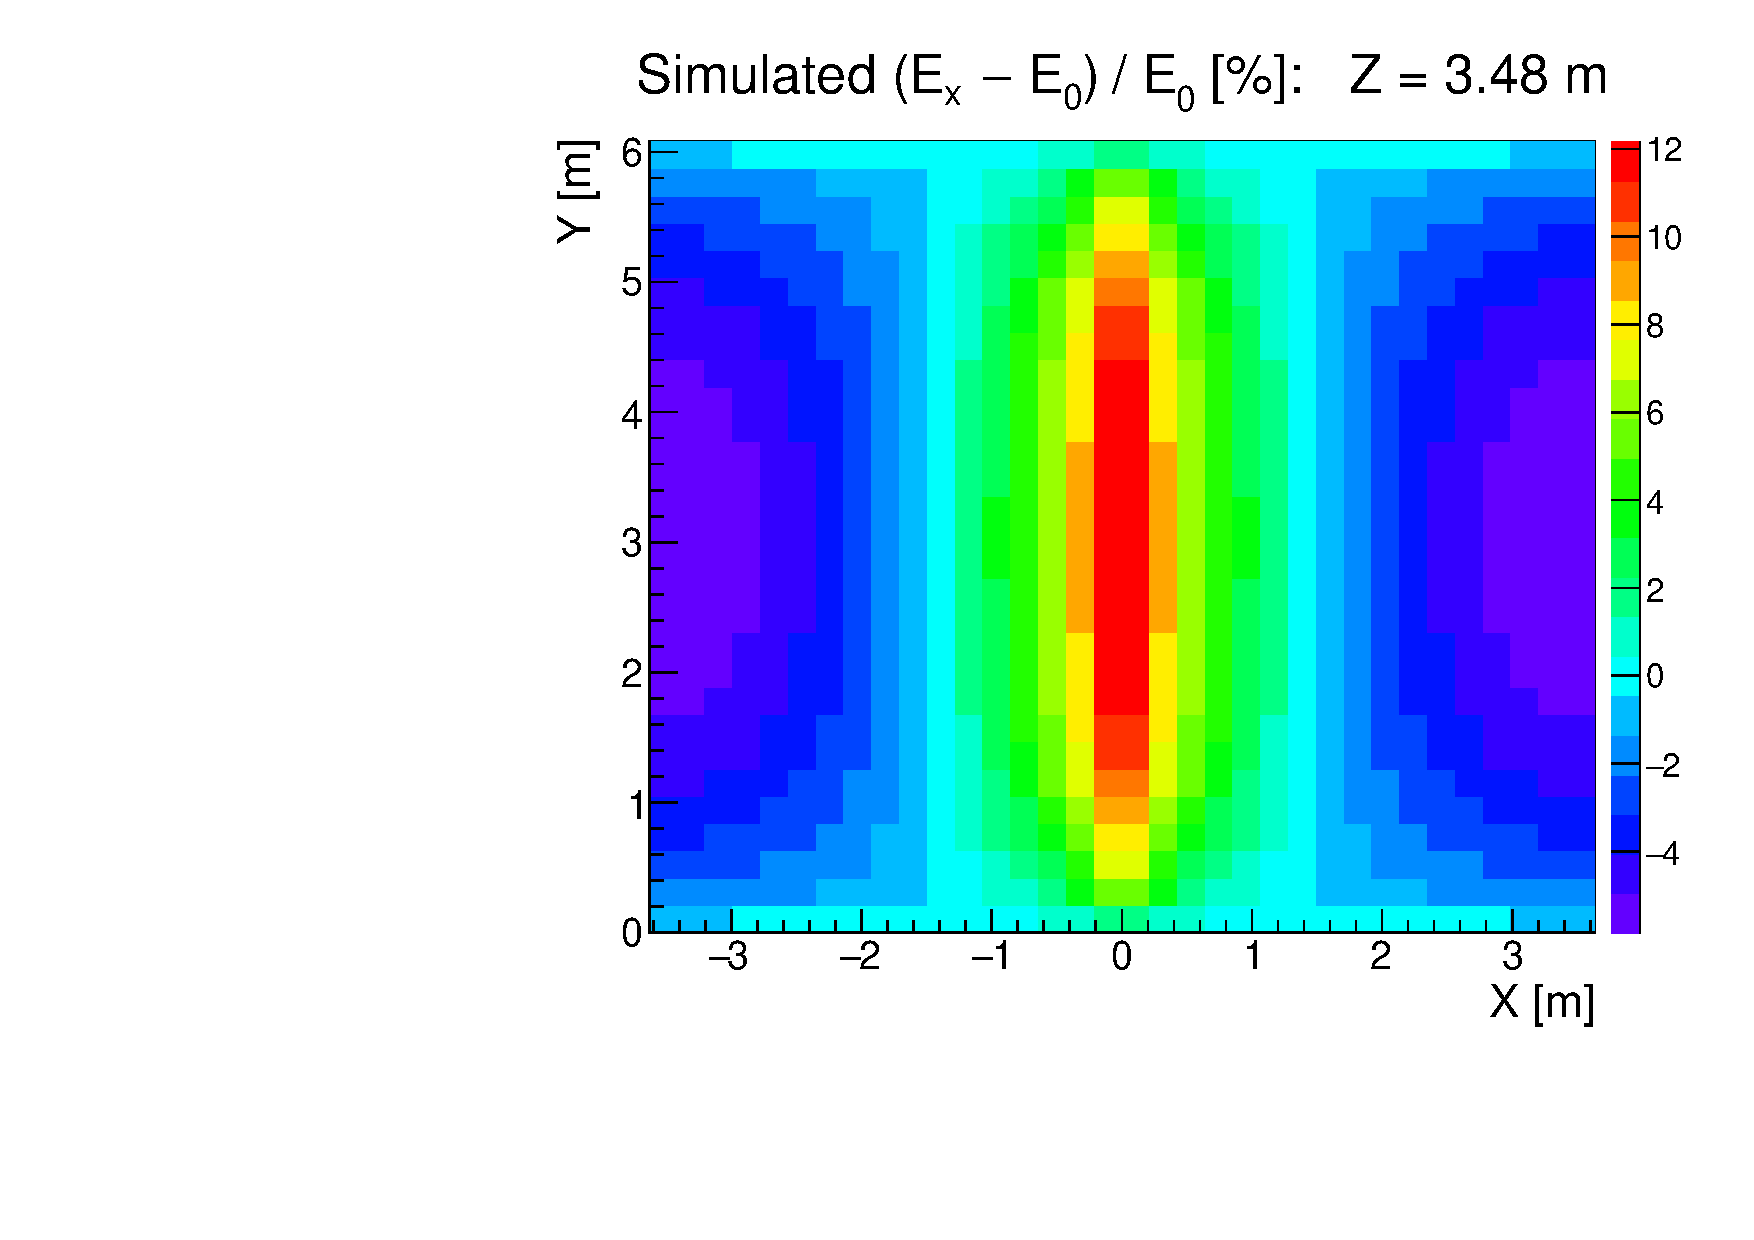
\includegraphics[width=.41\textwidth]{Ex_center_ProtoDUNE_E500.pdf}
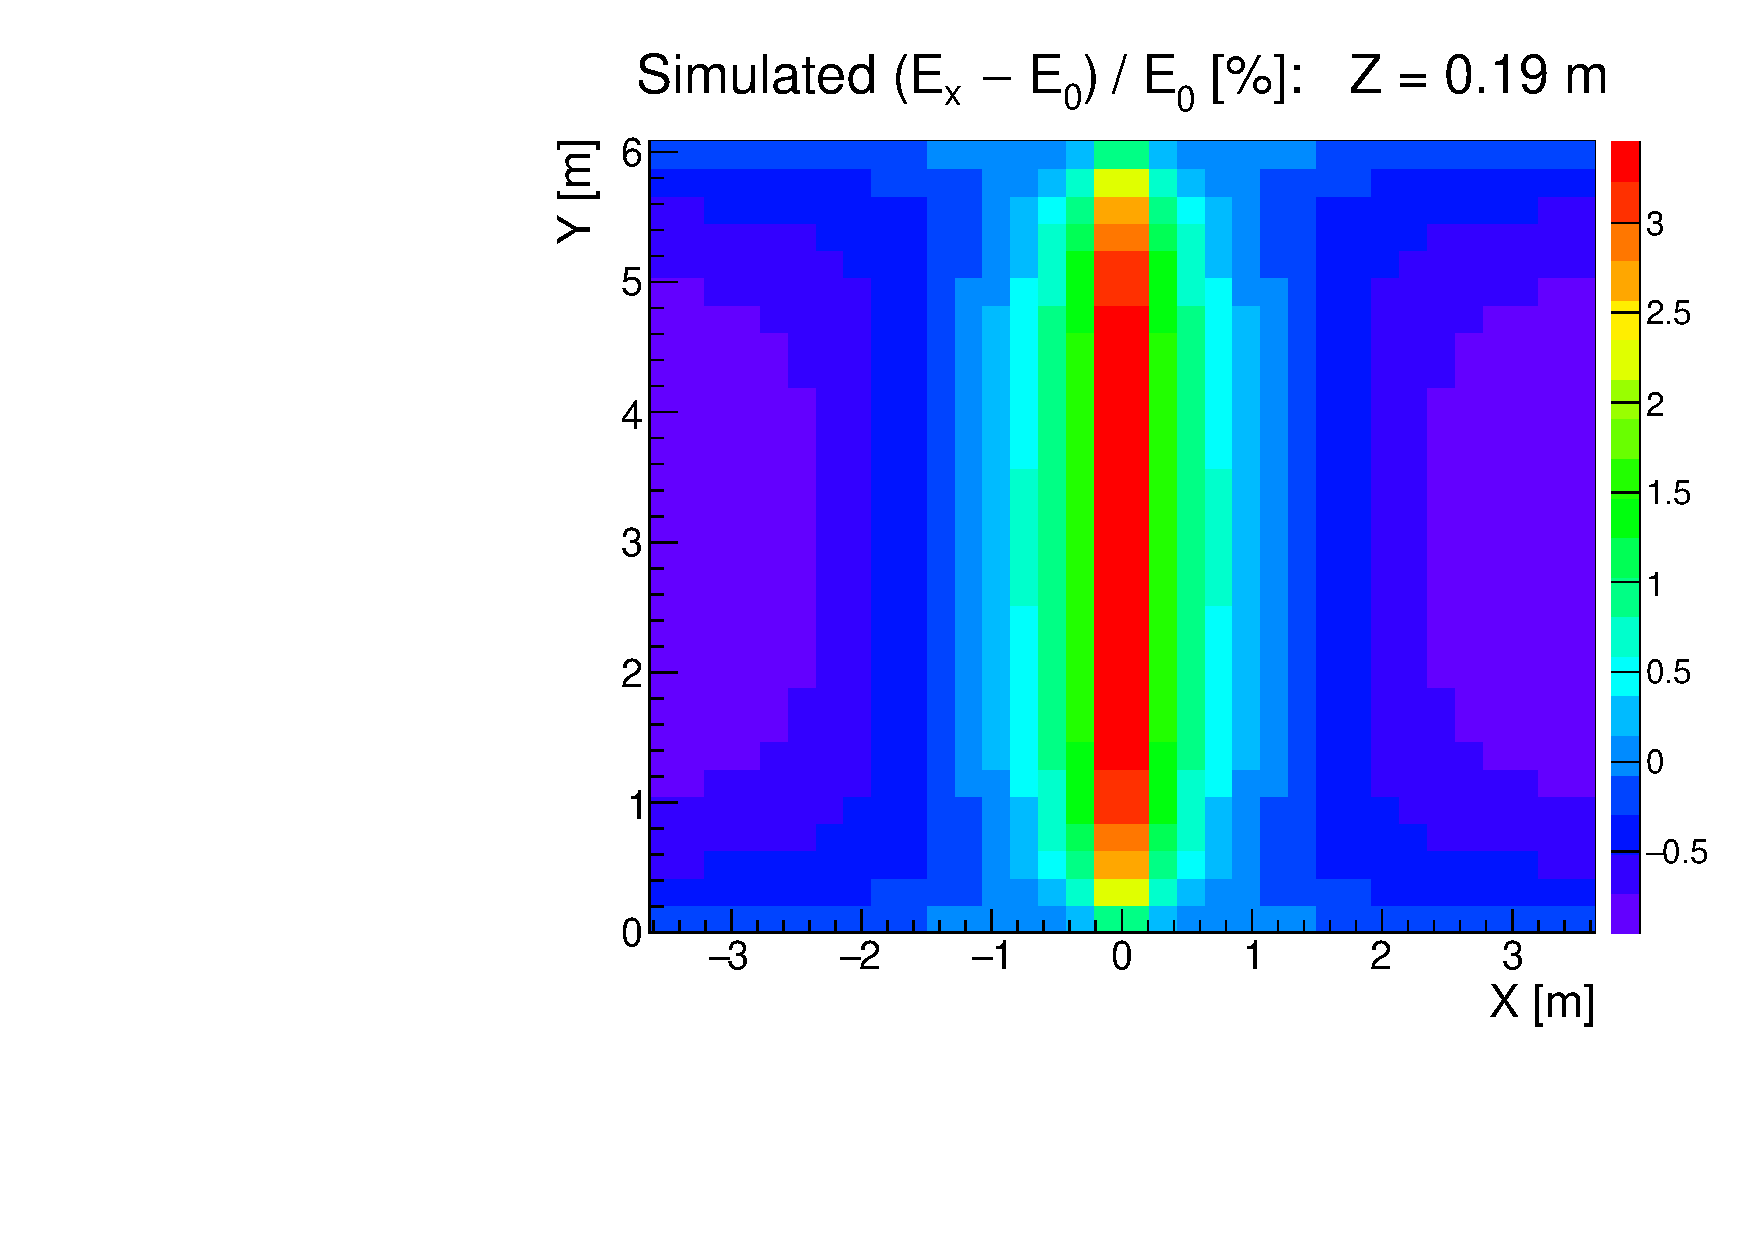
\includegraphics[width=.41\textwidth]{Ex_end_ProtoDUNE_E500.pdf}
\\
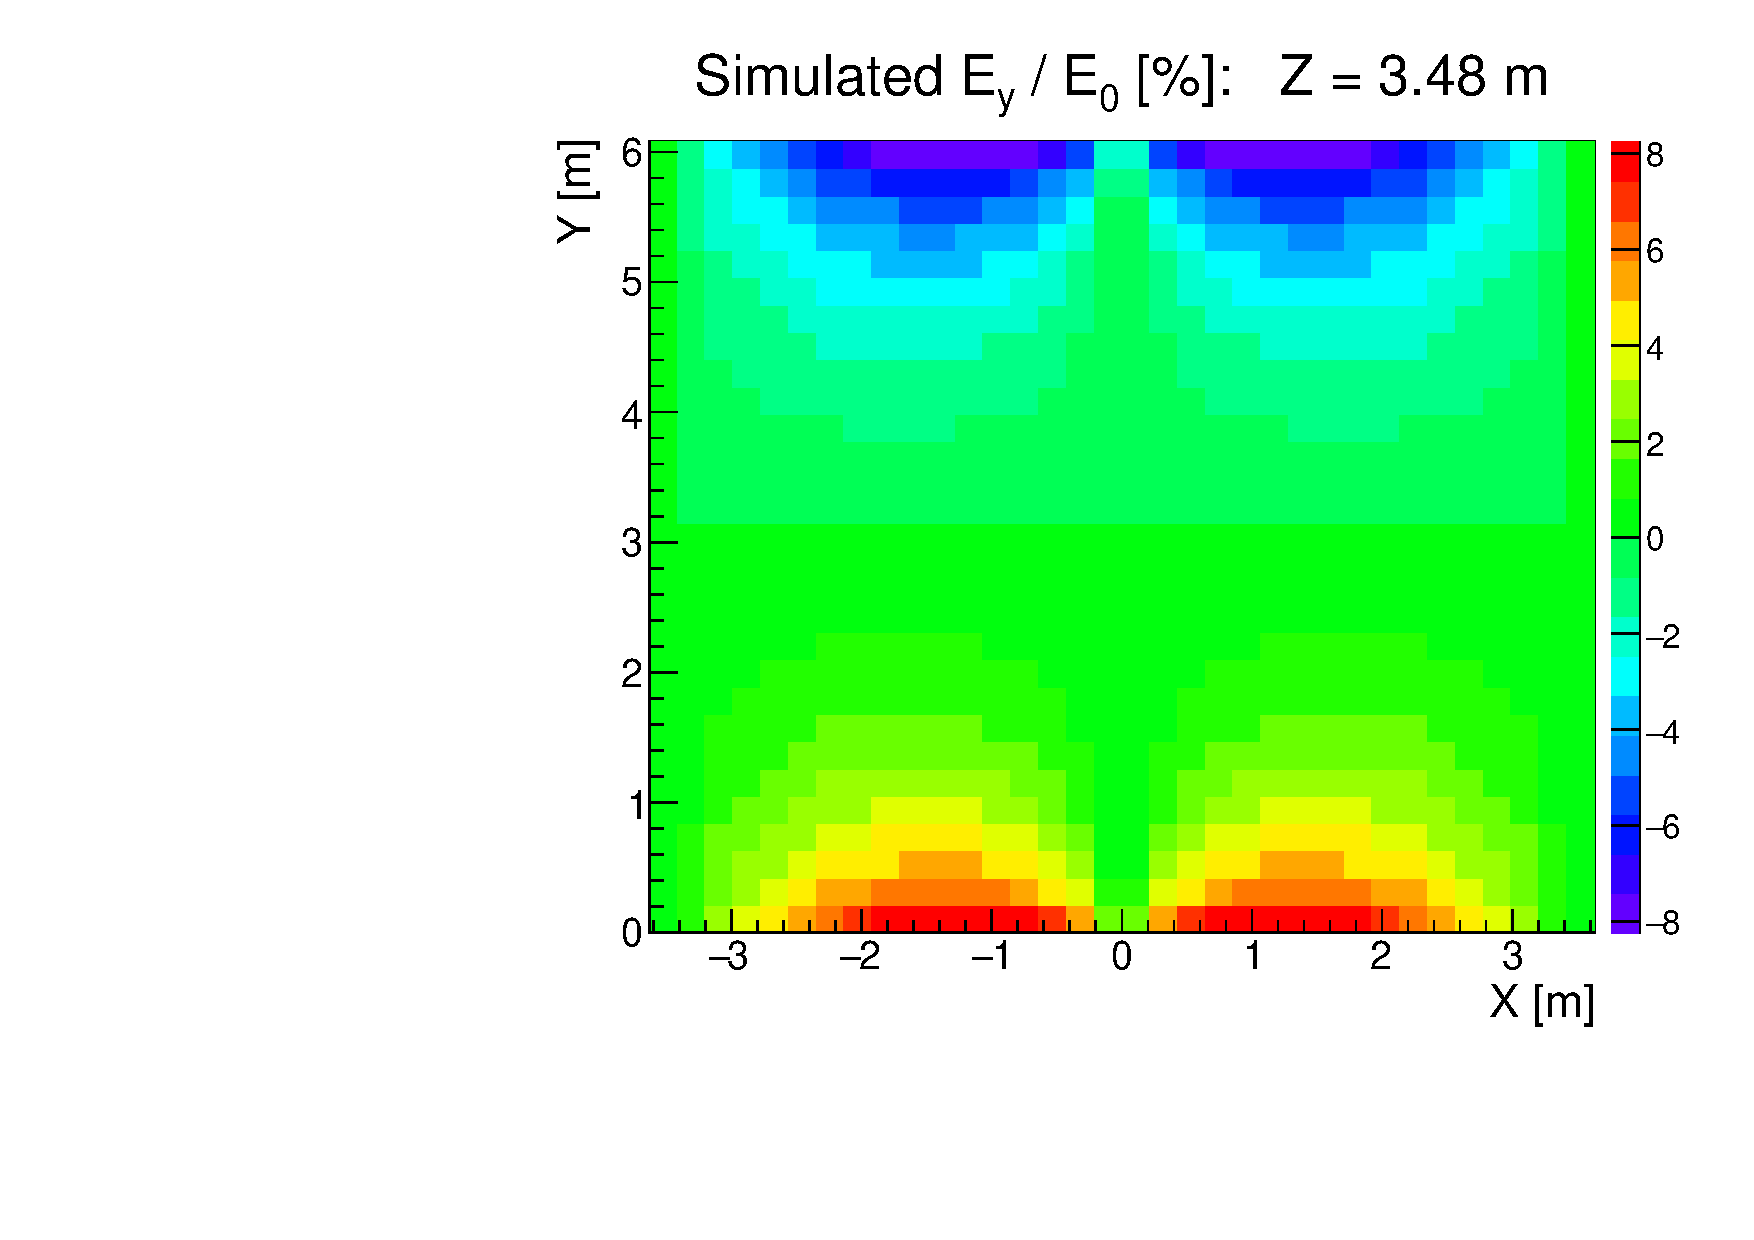
\includegraphics[width=.41\textwidth]{Ey_center_ProtoDUNE_E500.pdf}
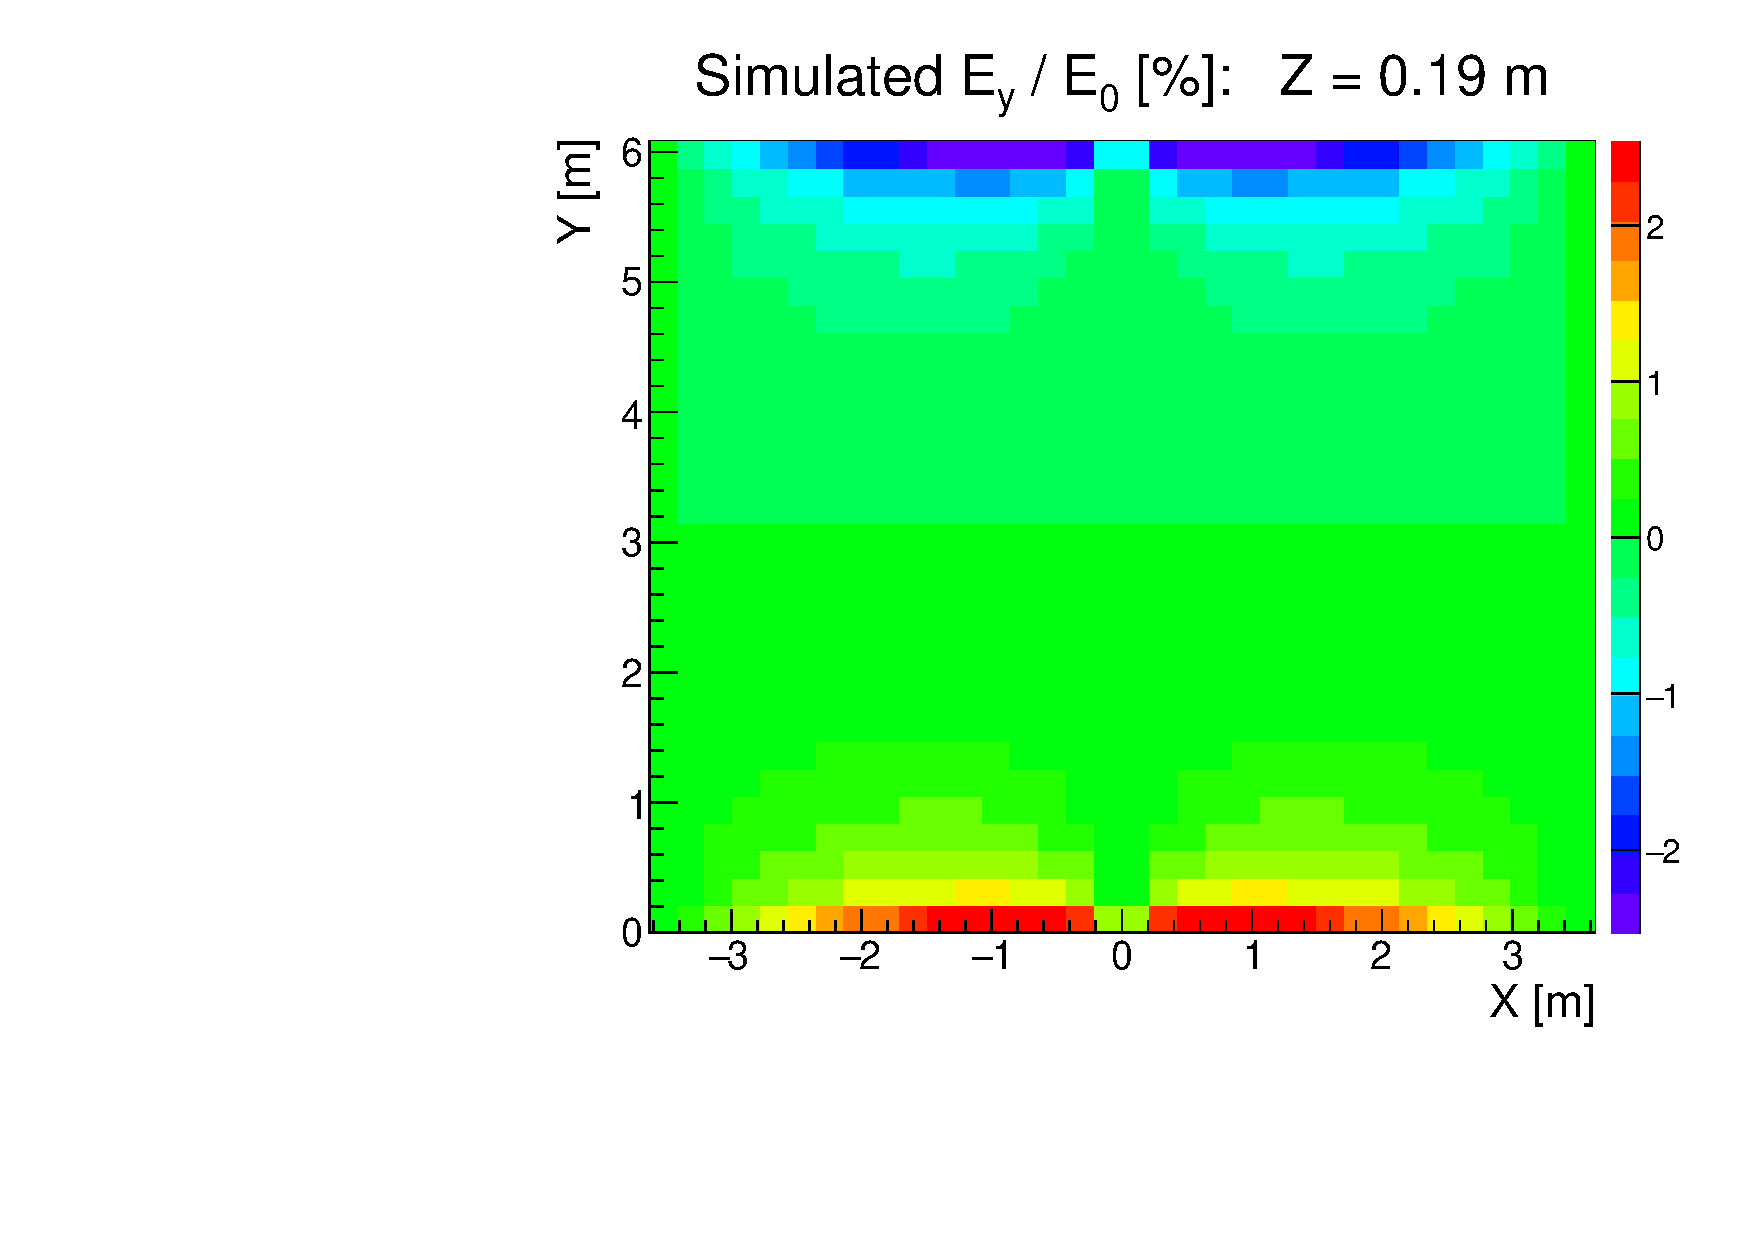
\includegraphics[width=.41\textwidth]{Ey_end_ProtoDUNE_E500.pdf}
\\
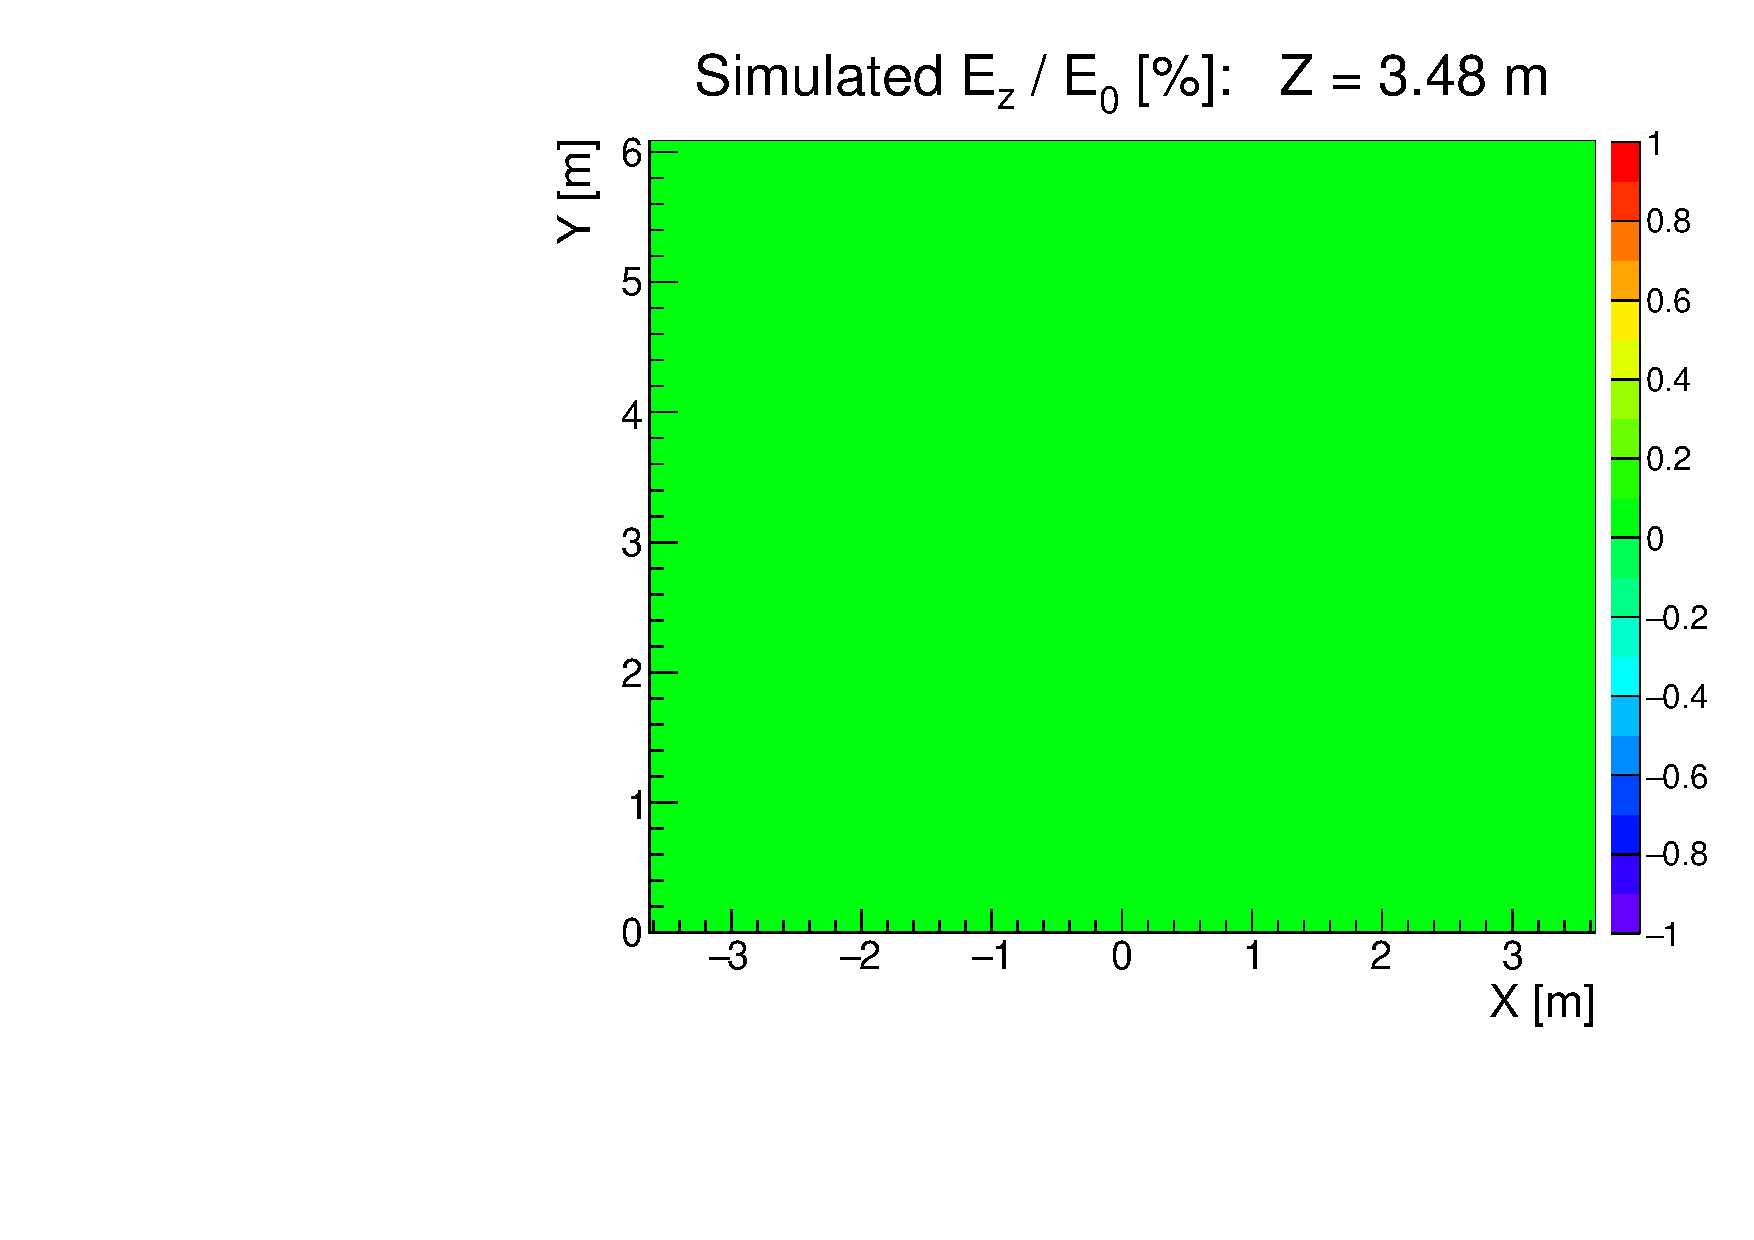
\includegraphics[width=.41\textwidth]{Ez_center_ProtoDUNE_E500.pdf}
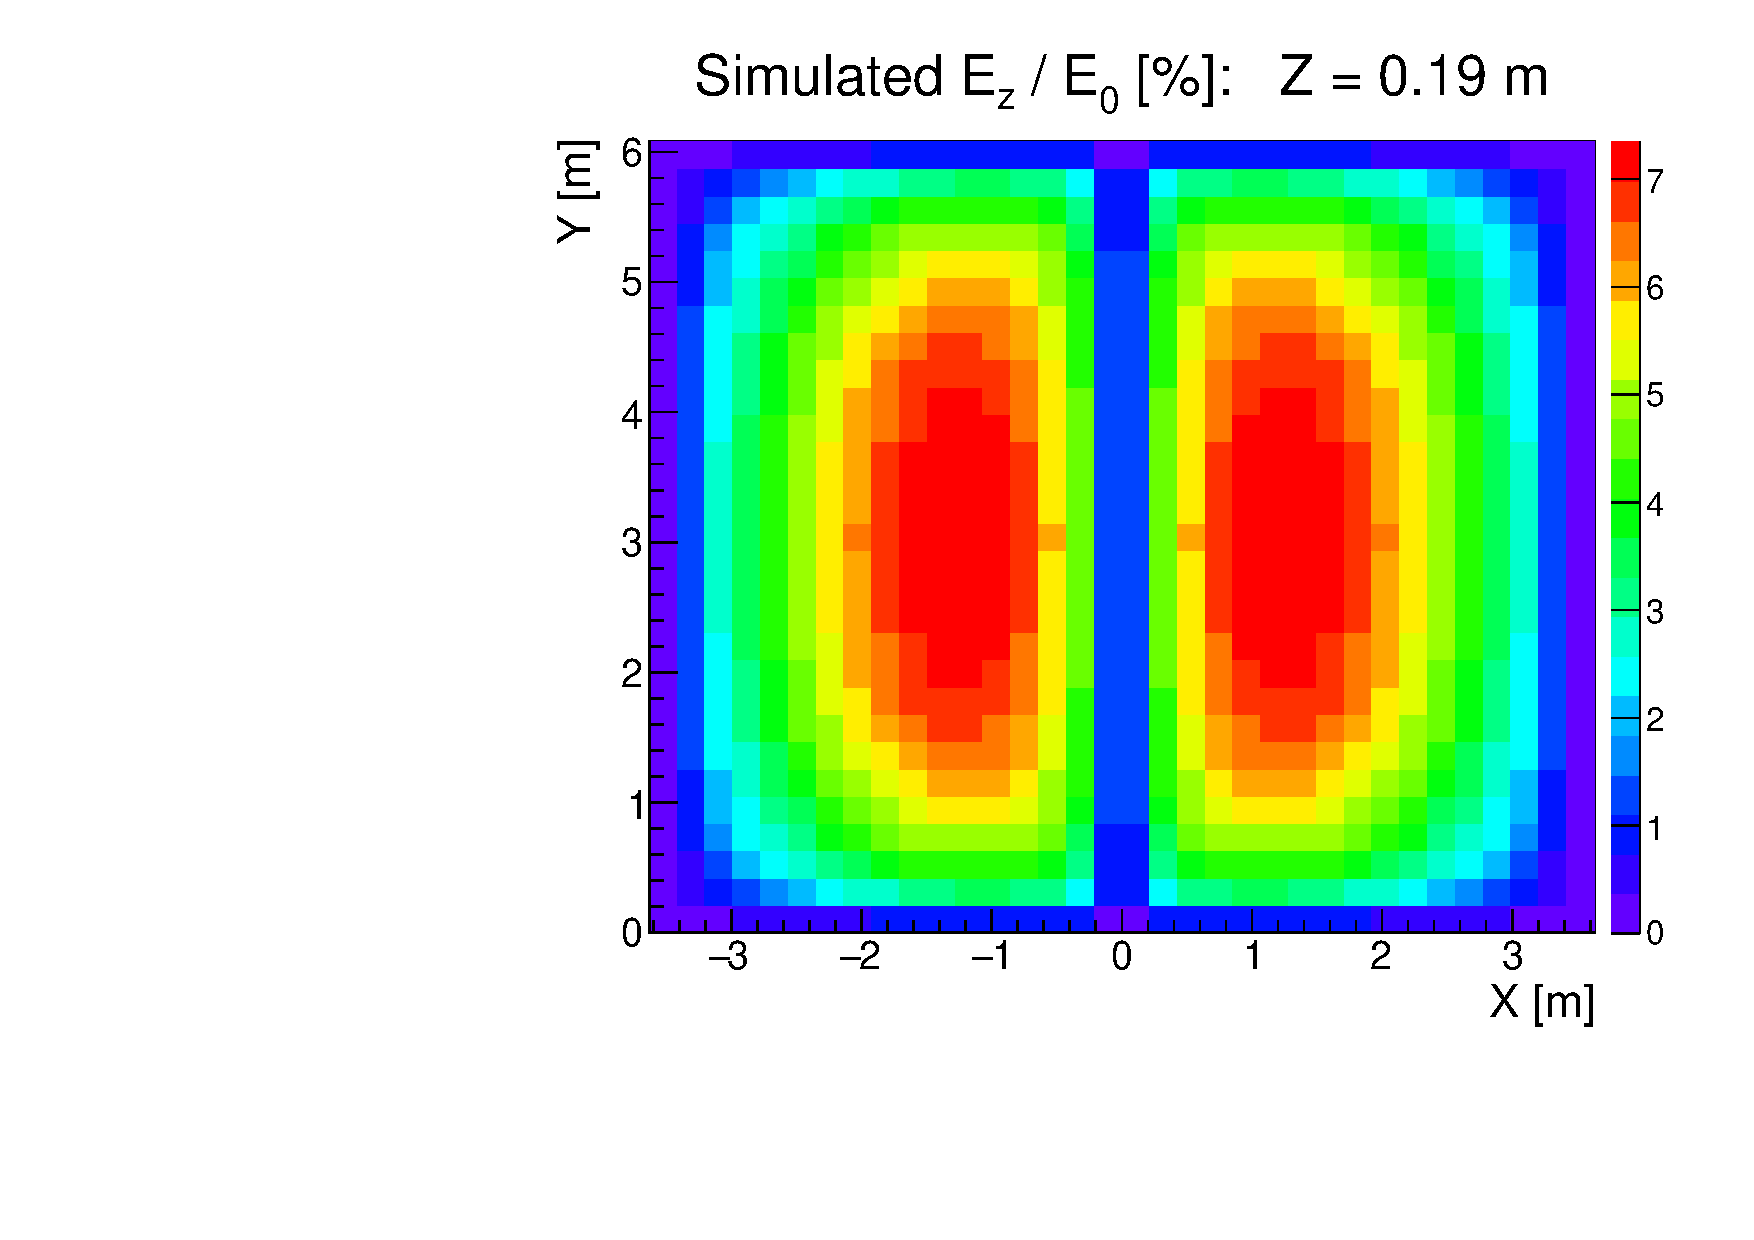
\includegraphics[width=.41\textwidth]{Ez_end_ProtoDUNE_E500.pdf}
\end{cdrfigure}


\begin{cdrfigure}[Simulated effects of space charge on distortions in recon ionization e- cluster position]{simexample_Dvals}{Illustration of the simulated effects of space charge on the distortions in reconstructed ionization electron cluster position in the ProtoDUNE-SP TPC.  Results are shown for the effect in $x$ (top row), $y$ (middle row), and $z$ (bottom row).  The distortions in reconstructed ionization electron cluster position are shown in units of cm and are plotted as a function of the true position in the TPC.  Simulation results are shown both for a central slice in $z$ (left column) and for a slice in $z$ closer to the end of the TPC, $z$ = 19 cm (right column).}
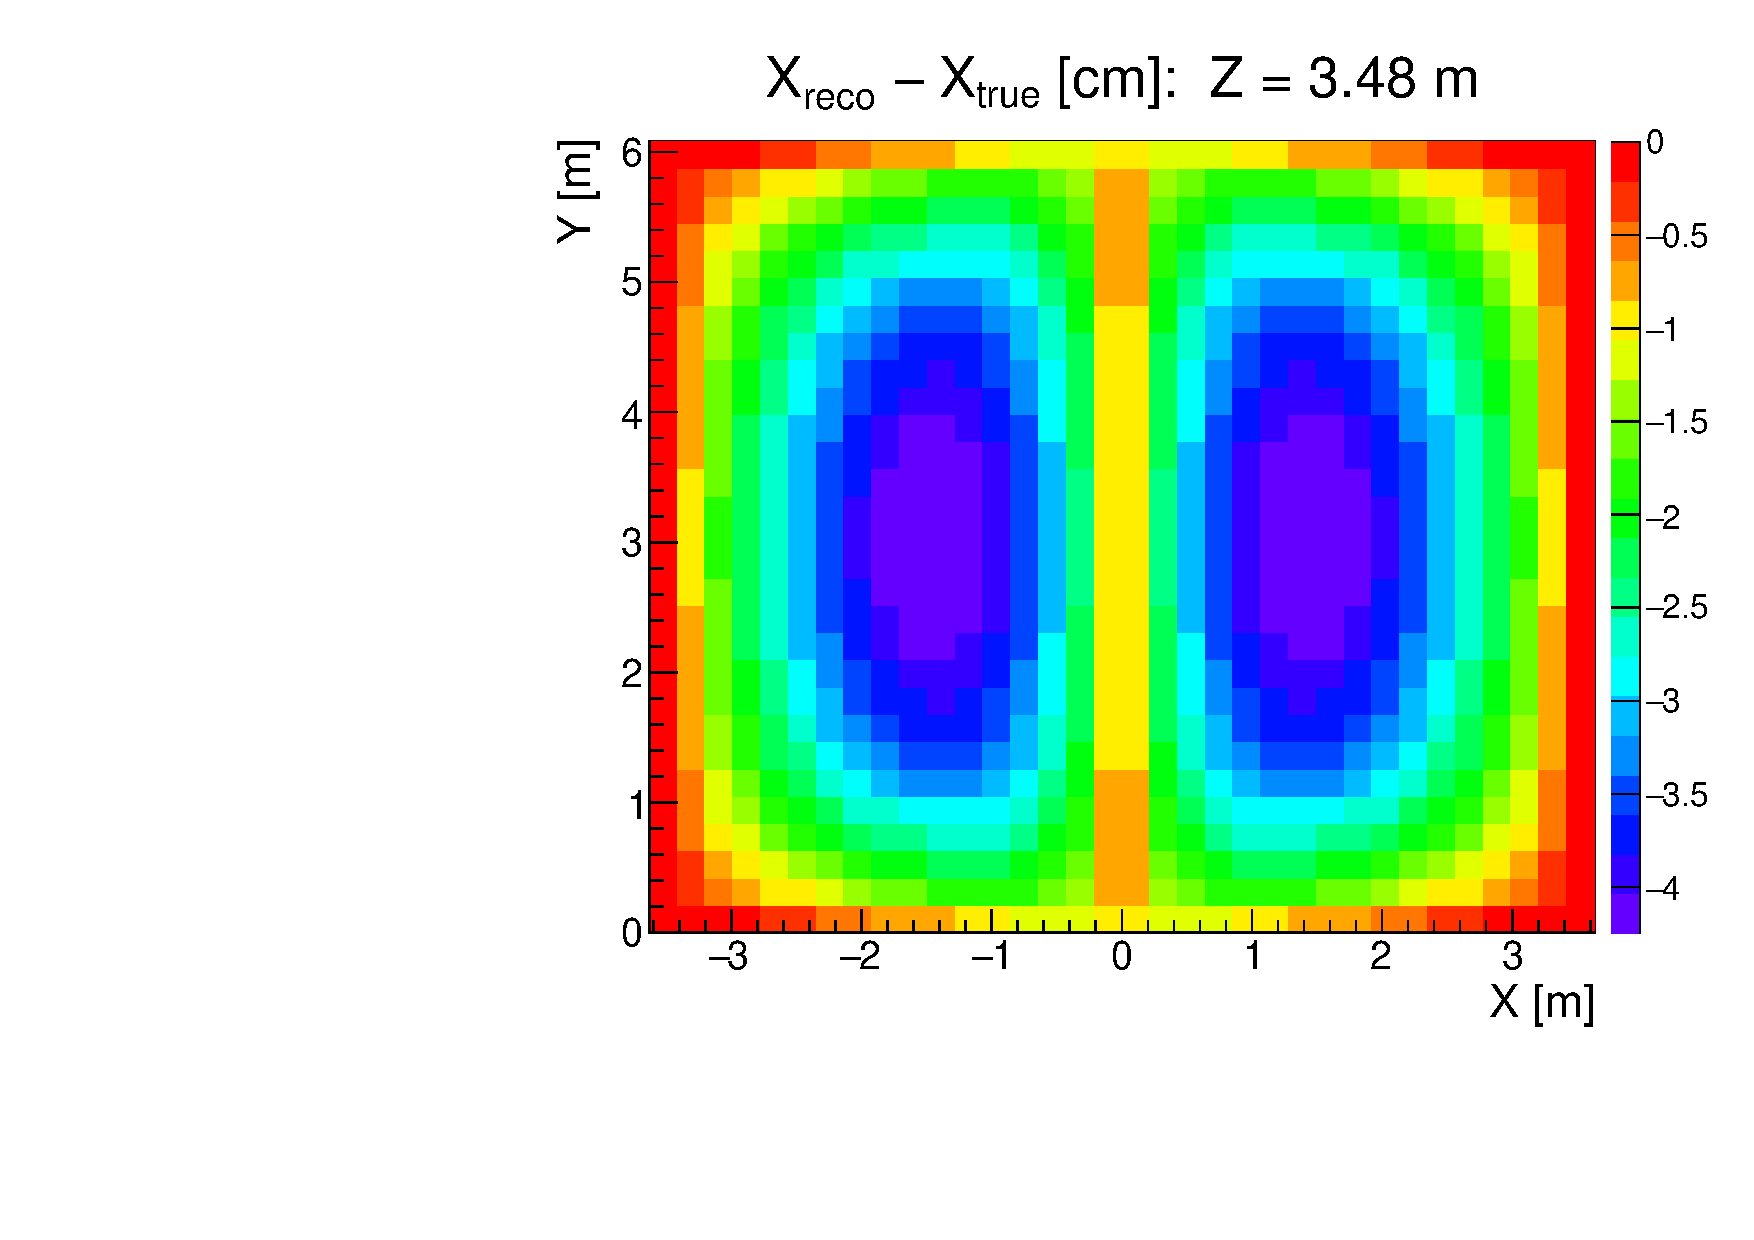
\includegraphics[width=.41\textwidth]{Dx_center_ProtoDUNE_E500.pdf}
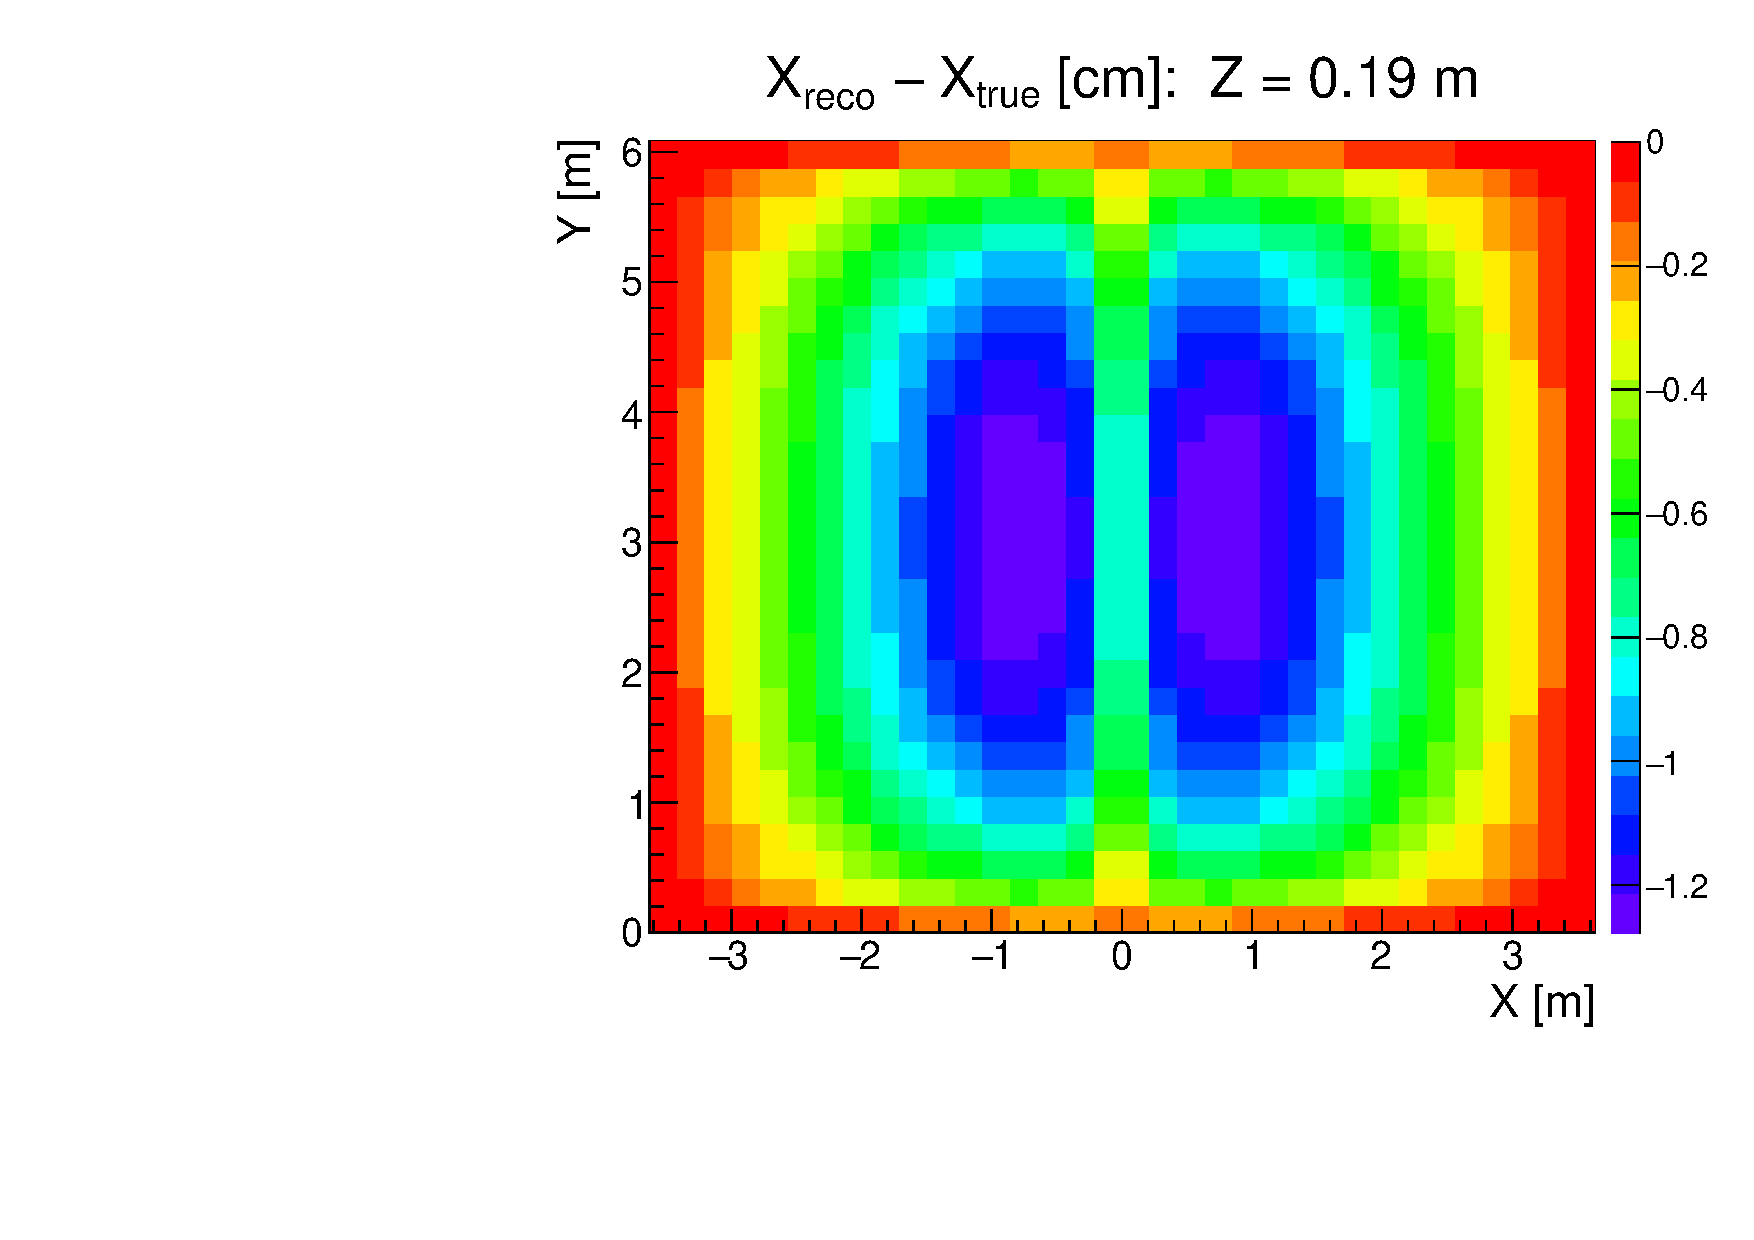
\includegraphics[width=.41\textwidth]{Dx_end_ProtoDUNE_E500.pdf}
\\
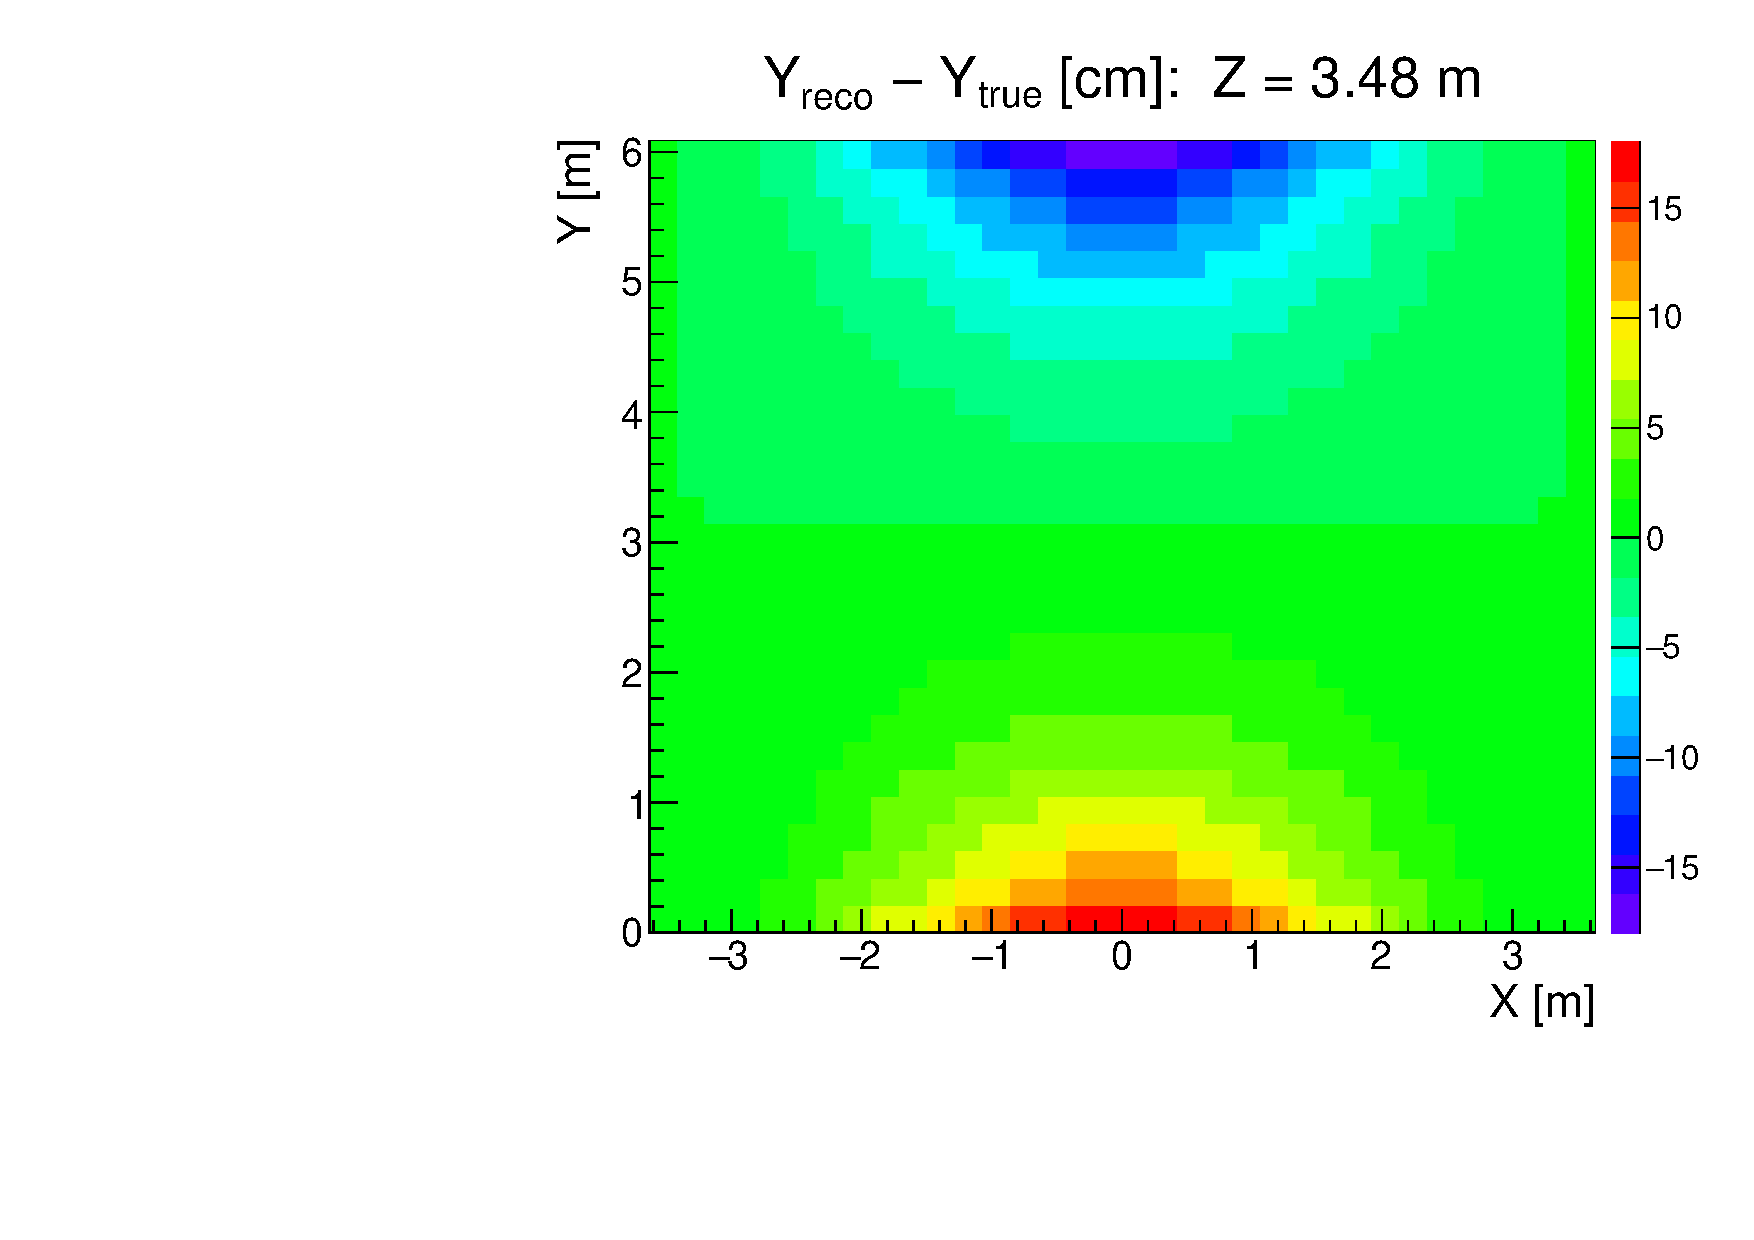
\includegraphics[width=.41\textwidth]{Dy_center_ProtoDUNE_E500.pdf}
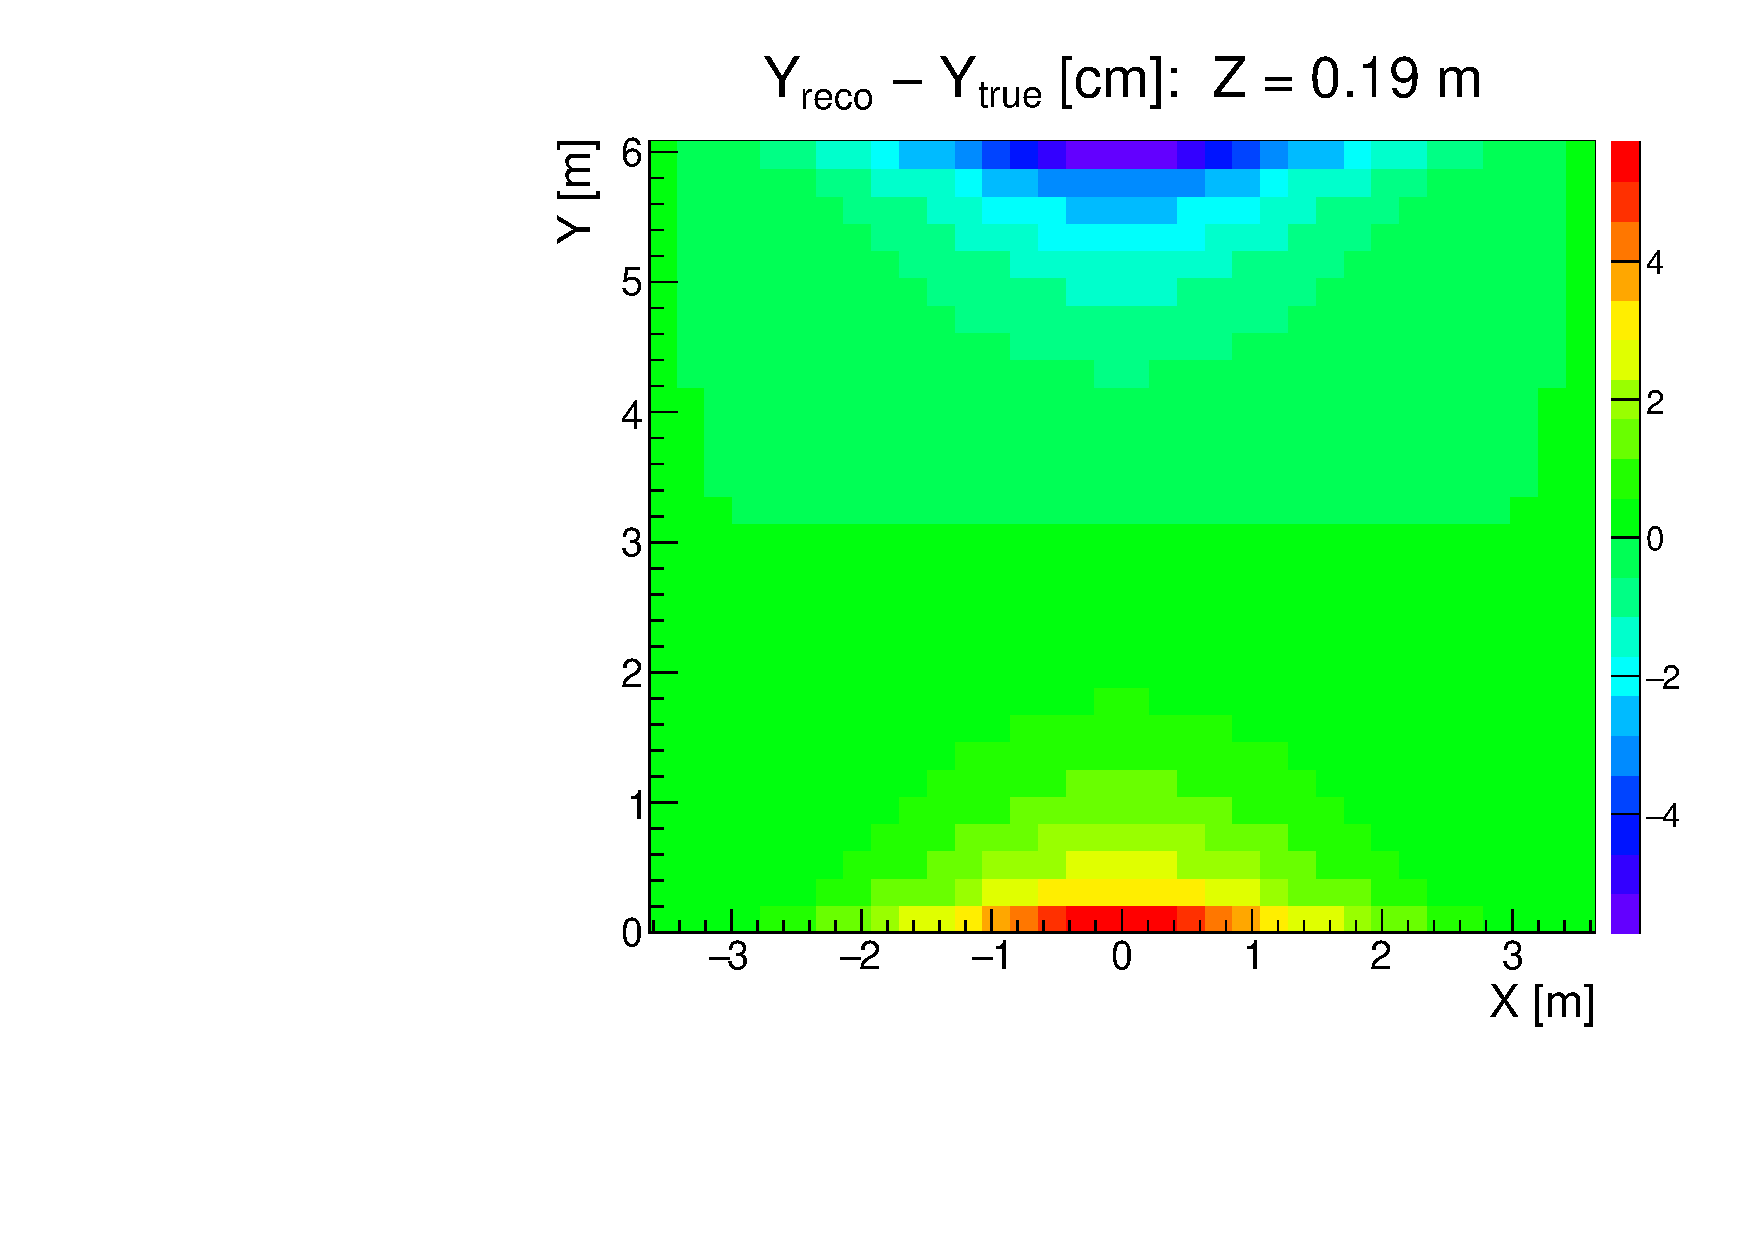
\includegraphics[width=.41\textwidth]{Dy_end_ProtoDUNE_E500.pdf}
\\
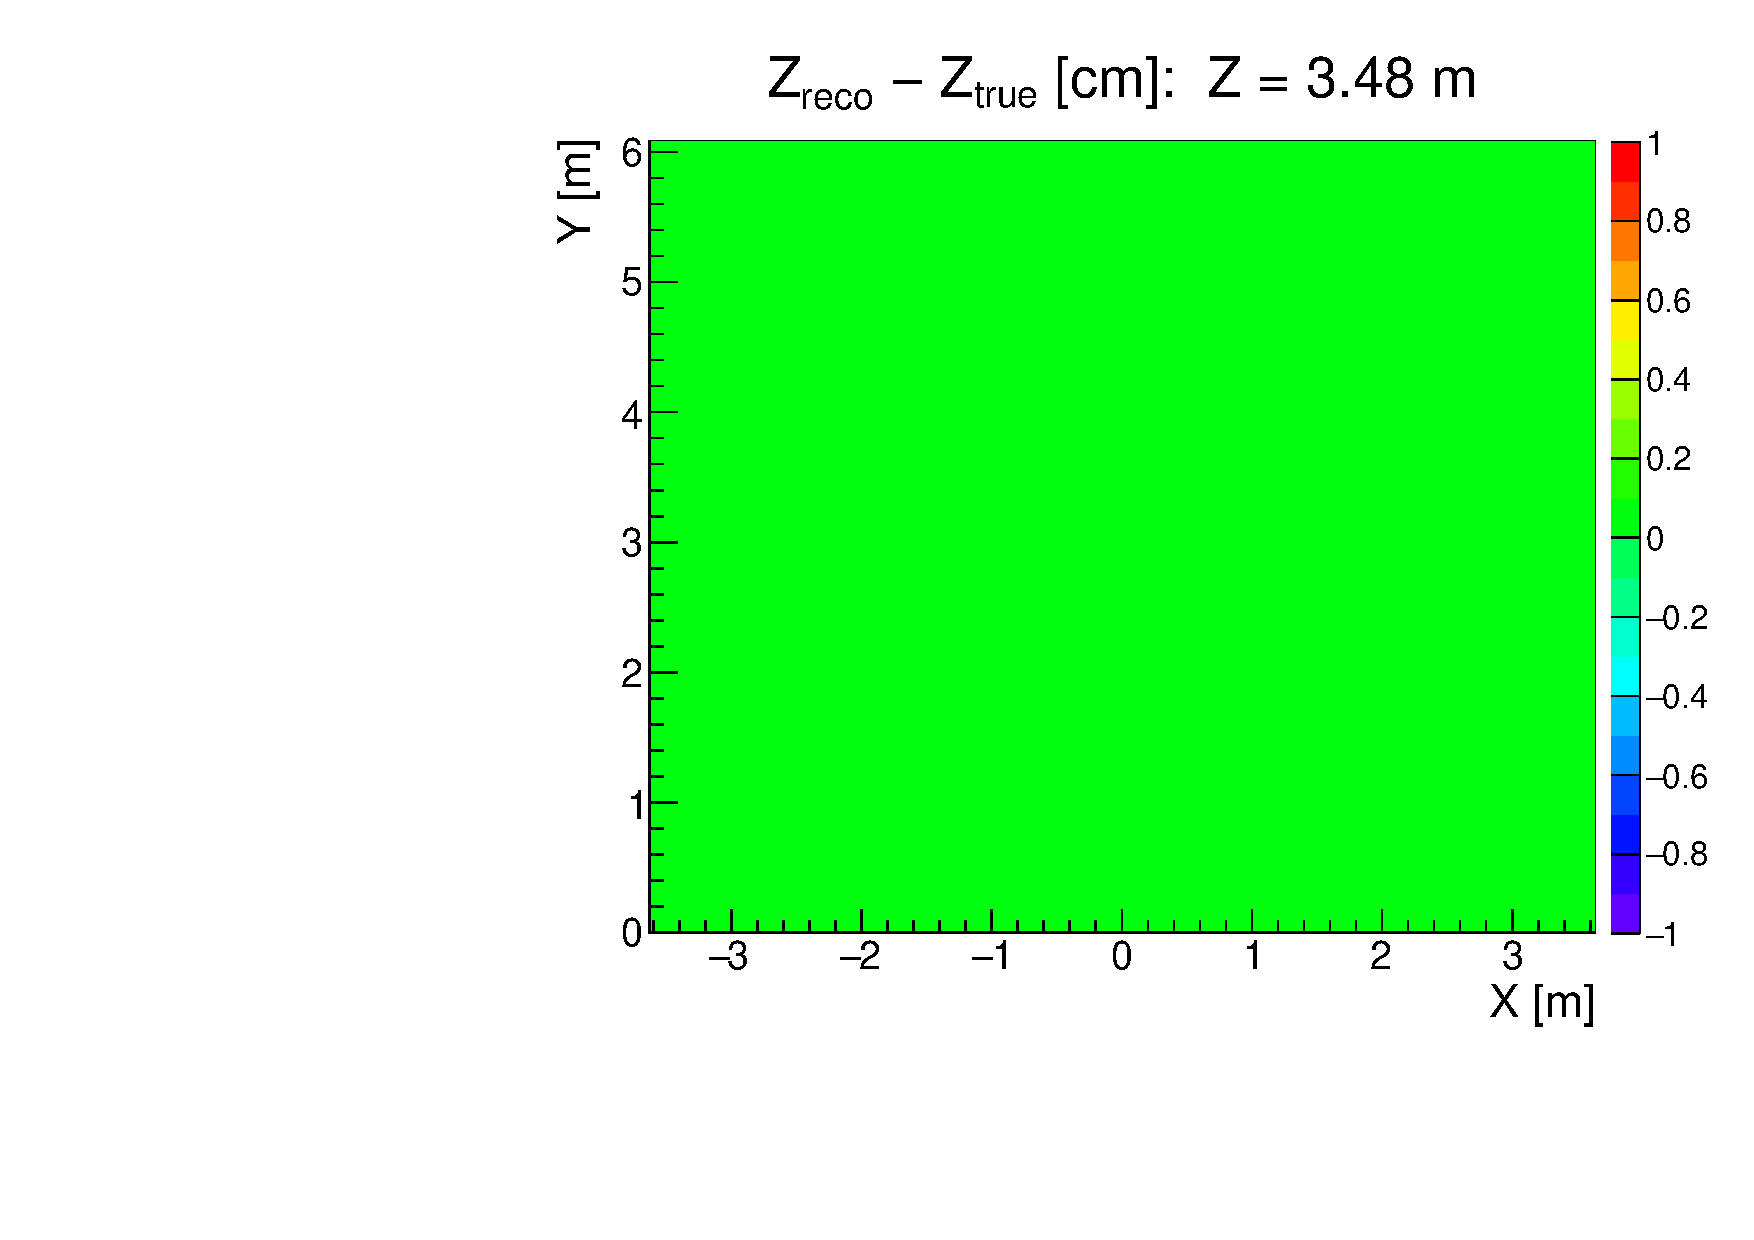
\includegraphics[width=.41\textwidth]{Dz_center_ProtoDUNE_E500.pdf}
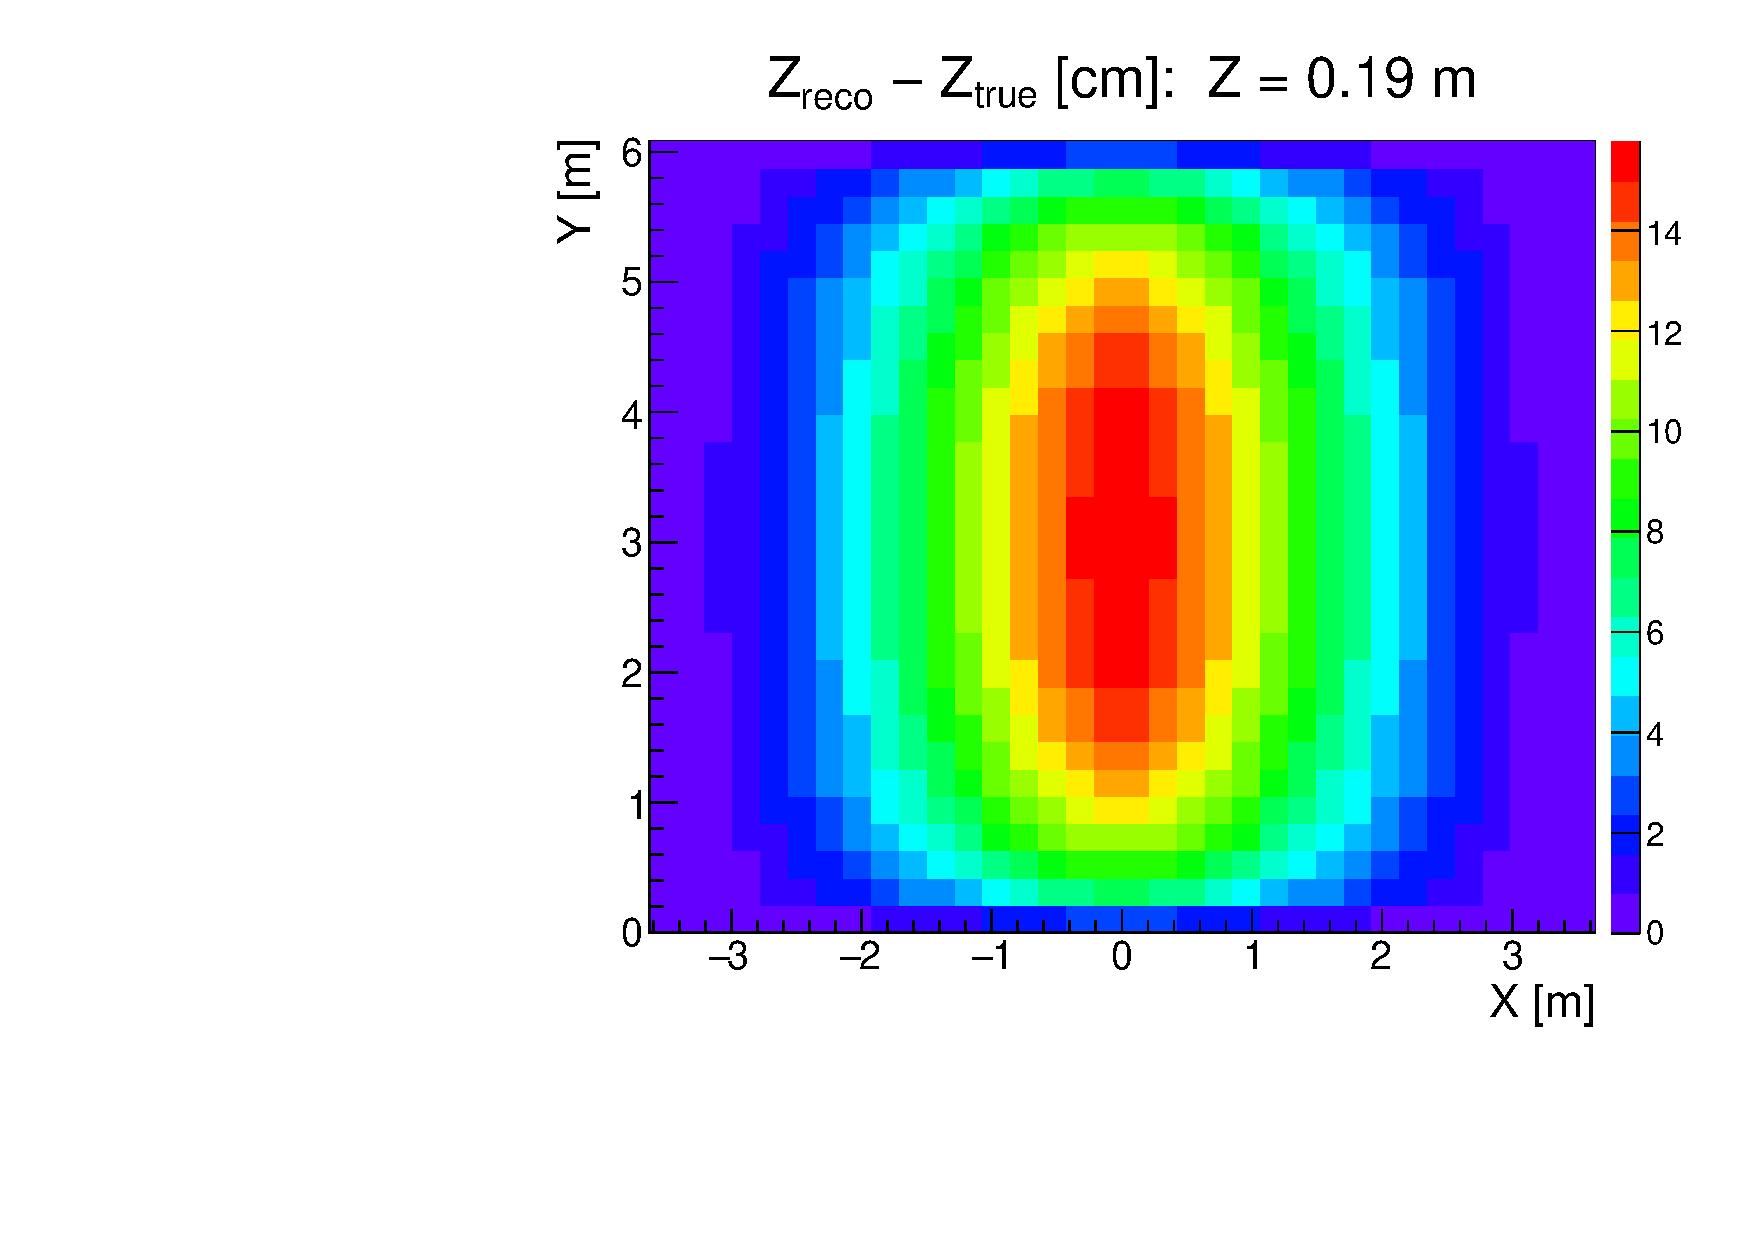
\includegraphics[width=.42\textwidth]{Dz_end_ProtoDUNE_E500.pdf}
\end{cdrfigure}



While the simulation provides a useful order-of-magnitude estimation of the distortions in electric field and reconstructed ionization electron cluster position within the ProtoDUNE-SP TPC, and provides basic shape features that we might expect in the data, there are several understood limitations of the simulation.  First of all, the flow of liquid argon, which may move positive argon ions in or out of the active TPC volume, is not considered.  Also, the assumption of uniform charge deposition from cosmics throughout the TPC may not be the case in reality, as enhanced cosmogenic activity near the top of the detector may lead to greater ion production rates closer to the top of the TPC active volume.  Finally, the linear space charge density assumed in the simulation (see Figure~\ref{fig:simSCDist}) is not quite correct; this approximates the ion drift speed (roughly 8~mm/s at a drift field of 500~V/cm) as constant throughout the TPC, while in reality the electric field distortions arising from the SCE itself would break this assumption.  With that in mind, comparisons of the simulation to first data collected at MicroBooNE show good agreement in terms of both magnitude and shape, looking at the top and bottom of the MicroBooNE TPC, with minor discrepancies due to what is believed to be effects of liquid argon flow moving space charge outside of the TPC active volume~\cite{SCEnoteMicroBooNE}.

%%%%%%%%%%%%%%%%%%%%%%%%
\subsection{Calibration} \label{sec:SCEcalib}

In order to correct SCE distortions (both electric field and reconstructed ionization electron cluster position) in data, a robust calibration scheme is necessary.  With information about the true position of ionization within the TPC in hand, as well as the reconstructed position of the ionization, spatial distortions of ionization deposition position can be extracted throughout the TPC active volume.  These spatial distortions can then be used to calculate the amount of electric field distortion throughout the TPC active volume.  Together, these two distortion maps can be used to correct track angles and calibrate out the variation in recombination and scintillation light yield throughout the TPC.

The strategy outlined above necessitates knowing both true and reconstructed ionization electron cluster positions throughout the TPC active volume.  This information can be obtained by using either cosmic muons or laser tracks.  In the case of cosmic muons, the ends of the tracks at the edges of the TPC active volume can be used to determine the spatial offsets due to SCE in the parts of the TPC where the transverse SCE is expected to be largest (see Figure~\ref{fig:simexample_Dvals}).  This first requires determining the $t_0$ of the cosmic muon, which can be obtained by either using a light-collection system or an external tagger (such as scintillator paddles located outside of the cryostat).  In the case of laser tracks, the true laser path through the TPC is known, allowing for calibration of spatial offsets due to SCE in the bulk of the TPC.  Together, cosmic muons and laser tracks (from e.g., a UV laser system installed at opposite ends of the cryostat~\cite{Ereditato:2014lra}) can be utilized to obtain SCE corrections throughout the entire TPC active volume.

Such calibration techniques discussed above require that the disortions due to SCE be relatively stable over time.  Preliminary observations at MicroBooNE suggest that this is the case on the timescale of several months~\cite{SCEnoteMicroBooNE}, though for a different cryogenic system.  This last point is important to note as the liquid argon flow pattern may be significantly different at ProtoDUNE-SP, leading to a space charge profile that may be time-dependent.

